\documentclass[twoside]{book}

% Packages required by doxygen
\usepackage{fixltx2e}
\usepackage{calc}
\usepackage{doxygen}
\usepackage[export]{adjustbox} % also loads graphicx
\usepackage{graphicx}
\usepackage[utf8]{inputenc}
\usepackage{makeidx}
\usepackage{multicol}
\usepackage{multirow}
\PassOptionsToPackage{warn}{textcomp}
\usepackage{textcomp}
\usepackage[nointegrals]{wasysym}
\usepackage[table]{xcolor}

% Font selection
\usepackage[T1]{fontenc}
\usepackage[scaled=.90]{helvet}
\usepackage{courier}
\usepackage{amssymb}
\usepackage{sectsty}
\renewcommand{\familydefault}{\sfdefault}
\allsectionsfont{%
  \fontseries{bc}\selectfont%
  \color{darkgray}%
}
\renewcommand{\DoxyLabelFont}{%
  \fontseries{bc}\selectfont%
  \color{darkgray}%
}
\newcommand{\+}{\discretionary{\mbox{\scriptsize$\hookleftarrow$}}{}{}}

% Page & text layout
\usepackage{geometry}
\geometry{%
  a4paper,%
  top=2.5cm,%
  bottom=2.5cm,%
  left=2.5cm,%
  right=2.5cm%
}
\tolerance=750
\hfuzz=15pt
\hbadness=750
\setlength{\emergencystretch}{15pt}
\setlength{\parindent}{0cm}
\setlength{\parskip}{3ex plus 2ex minus 2ex}
\makeatletter
\renewcommand{\paragraph}{%
  \@startsection{paragraph}{4}{0ex}{-1.0ex}{1.0ex}{%
    \normalfont\normalsize\bfseries\SS@parafont%
  }%
}
\renewcommand{\subparagraph}{%
  \@startsection{subparagraph}{5}{0ex}{-1.0ex}{1.0ex}{%
    \normalfont\normalsize\bfseries\SS@subparafont%
  }%
}
\makeatother

% Headers & footers
\usepackage{fancyhdr}
\pagestyle{fancyplain}
\fancyhead[LE]{\fancyplain{}{\bfseries\thepage}}
\fancyhead[CE]{\fancyplain{}{}}
\fancyhead[RE]{\fancyplain{}{\bfseries\leftmark}}
\fancyhead[LO]{\fancyplain{}{\bfseries\rightmark}}
\fancyhead[CO]{\fancyplain{}{}}
\fancyhead[RO]{\fancyplain{}{\bfseries\thepage}}
\fancyfoot[LE]{\fancyplain{}{}}
\fancyfoot[CE]{\fancyplain{}{}}
\fancyfoot[RE]{\fancyplain{}{\bfseries\scriptsize Generated by Doxygen }}
\fancyfoot[LO]{\fancyplain{}{\bfseries\scriptsize Generated by Doxygen }}
\fancyfoot[CO]{\fancyplain{}{}}
\fancyfoot[RO]{\fancyplain{}{}}
\renewcommand{\footrulewidth}{0.4pt}
\renewcommand{\chaptermark}[1]{%
  \markboth{#1}{}%
}
\renewcommand{\sectionmark}[1]{%
  \markright{\thesection\ #1}%
}

% Indices & bibliography
\usepackage{natbib}
\usepackage[titles]{tocloft}
\setcounter{tocdepth}{3}
\setcounter{secnumdepth}{5}
\makeindex

% Hyperlinks (required, but should be loaded last)
\usepackage{ifpdf}
\ifpdf
  \usepackage[pdftex,pagebackref=true]{hyperref}
\else
  \usepackage[ps2pdf,pagebackref=true]{hyperref}
\fi
\hypersetup{%
  colorlinks=true,%
  linkcolor=blue,%
  citecolor=blue,%
  unicode%
}

% Custom commands
\newcommand{\clearemptydoublepage}{%
  \newpage{\pagestyle{empty}\cleardoublepage}%
}

\usepackage{caption}
\captionsetup{labelsep=space,justification=centering,font={bf},singlelinecheck=off,skip=4pt,position=top}

%===== C O N T E N T S =====

\begin{document}

% Titlepage & ToC
\hypersetup{pageanchor=false,
             bookmarksnumbered=true,
             pdfencoding=unicode
            }
\pagenumbering{alph}
\begin{titlepage}
\vspace*{7cm}
\begin{center}%
{\Large My Project }\\
\vspace*{1cm}
{\large Generated by Doxygen 1.8.13}\\
\end{center}
\end{titlepage}
\clearemptydoublepage
\pagenumbering{roman}
\tableofcontents
\clearemptydoublepage
\pagenumbering{arabic}
\hypersetup{pageanchor=true}

%--- Begin generated contents ---
\chapter{Hierarchical Index}
\section{Class Hierarchy}
This inheritance list is sorted roughly, but not completely, alphabetically\+:\begin{DoxyCompactList}
\item \contentsline{section}{backend.\+serializers.\+Enterprise\+Display\+Info\+Serializer.\+Meta}{\pageref{classbackend_1_1serializers_1_1_enterprise_display_info_serializer_1_1_meta}}{}
\item \contentsline{section}{backend.\+serializers.\+Customer\+Service\+Serializer.\+Meta}{\pageref{classbackend_1_1serializers_1_1_customer_service_serializer_1_1_meta}}{}
\item \contentsline{section}{backend.\+serializers.\+Chatting\+Log\+Serializer.\+Meta}{\pageref{classbackend_1_1serializers_1_1_chatting_log_serializer_1_1_meta}}{}
\item \contentsline{section}{backend.\+serializers.\+Serial\+Number\+Serializer.\+Meta}{\pageref{classbackend_1_1serializers_1_1_serial_number_serializer_1_1_meta}}{}
\item \contentsline{section}{backend.\+serializers.\+Big\+Image\+Log\+Serializer.\+Meta}{\pageref{classbackend_1_1serializers_1_1_big_image_log_serializer_1_1_meta}}{}
\item \contentsline{section}{backend.\+serializers.\+Small\+Image\+Log\+Serializer.\+Meta}{\pageref{classbackend_1_1serializers_1_1_small_image_log_serializer_1_1_meta}}{}
\item \contentsline{section}{backend.\+serializers.\+Customer\+Service\+Create\+Serializer.\+Meta}{\pageref{classbackend_1_1serializers_1_1_customer_service_create_serializer_1_1_meta}}{}
\item \contentsline{section}{backend.\+serializers.\+Admin\+Serializer.\+Meta}{\pageref{classbackend_1_1serializers_1_1_admin_serializer_1_1_meta}}{}
\item \contentsline{section}{backend.\+serializers.\+Robot\+Info\+Serializer.\+Meta}{\pageref{classbackend_1_1serializers_1_1_robot_info_serializer_1_1_meta}}{}
\item Model\begin{DoxyCompactList}
\item \contentsline{section}{backend.\+models.\+Admin}{\pageref{classbackend_1_1models_1_1_admin}}{}
\item \contentsline{section}{backend.\+models.\+Big\+Image\+Log}{\pageref{classbackend_1_1models_1_1_big_image_log}}{}
\item \contentsline{section}{backend.\+models.\+Chatting\+Log}{\pageref{classbackend_1_1models_1_1_chatting_log}}{}
\item \contentsline{section}{backend.\+models.\+Customer\+Service}{\pageref{classbackend_1_1models_1_1_customer_service}}{}
\item \contentsline{section}{backend.\+models.\+Enterprise\+Display\+Info}{\pageref{classbackend_1_1models_1_1_enterprise_display_info}}{}
\item \contentsline{section}{backend.\+models.\+Robot\+Gossip\+Info}{\pageref{classbackend_1_1models_1_1_robot_gossip_info}}{}
\item \contentsline{section}{backend.\+models.\+Robot\+Info}{\pageref{classbackend_1_1models_1_1_robot_info}}{}
\item \contentsline{section}{backend.\+models.\+Serial\+Number}{\pageref{classbackend_1_1models_1_1_serial_number}}{}
\item \contentsline{section}{backend.\+models.\+Small\+Image\+Log}{\pageref{classbackend_1_1models_1_1_small_image_log}}{}
\end{DoxyCompactList}
\item Model\+Serializer\begin{DoxyCompactList}
\item \contentsline{section}{backend.\+serializers.\+Admin\+Serializer}{\pageref{classbackend_1_1serializers_1_1_admin_serializer}}{}
\item \contentsline{section}{backend.\+serializers.\+Big\+Image\+Log\+Serializer}{\pageref{classbackend_1_1serializers_1_1_big_image_log_serializer}}{}
\item \contentsline{section}{backend.\+serializers.\+Chatting\+Log\+Serializer}{\pageref{classbackend_1_1serializers_1_1_chatting_log_serializer}}{}
\item \contentsline{section}{backend.\+serializers.\+Customer\+Service\+Create\+Serializer}{\pageref{classbackend_1_1serializers_1_1_customer_service_create_serializer}}{}
\item \contentsline{section}{backend.\+serializers.\+Customer\+Service\+Serializer}{\pageref{classbackend_1_1serializers_1_1_customer_service_serializer}}{}
\item \contentsline{section}{backend.\+serializers.\+Enterprise\+Display\+Info\+Serializer}{\pageref{classbackend_1_1serializers_1_1_enterprise_display_info_serializer}}{}
\item \contentsline{section}{backend.\+serializers.\+Robot\+Info\+Serializer}{\pageref{classbackend_1_1serializers_1_1_robot_info_serializer}}{}
\item \contentsline{section}{backend.\+serializers.\+Serial\+Number\+Serializer}{\pageref{classbackend_1_1serializers_1_1_serial_number_serializer}}{}
\item \contentsline{section}{backend.\+serializers.\+Small\+Image\+Log\+Serializer}{\pageref{classbackend_1_1serializers_1_1_small_image_log_serializer}}{}
\end{DoxyCompactList}
\item object\begin{DoxyCompactList}
\item \contentsline{section}{backend.\+models\+\_\+helper\+\_\+functions.\+Path\+And\+Rename}{\pageref{classbackend_1_1models__helper__functions_1_1_path_and_rename}}{}
\end{DoxyCompactList}
\item App\+Config\begin{DoxyCompactList}
\item \contentsline{section}{backend.\+apps.\+Backend\+Config}{\pageref{classbackend_1_1apps_1_1_backend_config}}{}
\end{DoxyCompactList}
\end{DoxyCompactList}

\chapter{Class Index}
\section{Class List}
Here are the classes, structs, unions and interfaces with brief descriptions\+:\begin{DoxyCompactList}
\item\contentsline{section}{\hyperlink{classbackend_1_1models_1_1_admin}{backend.\+models.\+Admin} }{\pageref{classbackend_1_1models_1_1_admin}}{}
\item\contentsline{section}{\hyperlink{classbackend_1_1serializers_1_1_admin_serializer}{backend.\+serializers.\+Admin\+Serializer} }{\pageref{classbackend_1_1serializers_1_1_admin_serializer}}{}
\item\contentsline{section}{\hyperlink{classbackend_1_1apps_1_1_backend_config}{backend.\+apps.\+Backend\+Config} }{\pageref{classbackend_1_1apps_1_1_backend_config}}{}
\item\contentsline{section}{\hyperlink{classbackend_1_1models_1_1_big_image_log}{backend.\+models.\+Big\+Image\+Log} }{\pageref{classbackend_1_1models_1_1_big_image_log}}{}
\item\contentsline{section}{\hyperlink{classbackend_1_1serializers_1_1_big_image_log_serializer}{backend.\+serializers.\+Big\+Image\+Log\+Serializer} }{\pageref{classbackend_1_1serializers_1_1_big_image_log_serializer}}{}
\item\contentsline{section}{\hyperlink{classbackend_1_1models_1_1_chatting_log}{backend.\+models.\+Chatting\+Log} }{\pageref{classbackend_1_1models_1_1_chatting_log}}{}
\item\contentsline{section}{\hyperlink{classbackend_1_1serializers_1_1_chatting_log_serializer}{backend.\+serializers.\+Chatting\+Log\+Serializer} }{\pageref{classbackend_1_1serializers_1_1_chatting_log_serializer}}{}
\item\contentsline{section}{\hyperlink{classbackend_1_1models_1_1_customer_service}{backend.\+models.\+Customer\+Service} }{\pageref{classbackend_1_1models_1_1_customer_service}}{}
\item\contentsline{section}{\hyperlink{classbackend_1_1serializers_1_1_customer_service_create_serializer}{backend.\+serializers.\+Customer\+Service\+Create\+Serializer} }{\pageref{classbackend_1_1serializers_1_1_customer_service_create_serializer}}{}
\item\contentsline{section}{\hyperlink{classbackend_1_1serializers_1_1_customer_service_serializer}{backend.\+serializers.\+Customer\+Service\+Serializer} }{\pageref{classbackend_1_1serializers_1_1_customer_service_serializer}}{}
\item\contentsline{section}{\hyperlink{classbackend_1_1models_1_1_enterprise_display_info}{backend.\+models.\+Enterprise\+Display\+Info} }{\pageref{classbackend_1_1models_1_1_enterprise_display_info}}{}
\item\contentsline{section}{\hyperlink{classbackend_1_1serializers_1_1_enterprise_display_info_serializer}{backend.\+serializers.\+Enterprise\+Display\+Info\+Serializer} }{\pageref{classbackend_1_1serializers_1_1_enterprise_display_info_serializer}}{}
\item\contentsline{section}{\hyperlink{classbackend_1_1serializers_1_1_enterprise_display_info_serializer_1_1_meta}{backend.\+serializers.\+Enterprise\+Display\+Info\+Serializer.\+Meta} }{\pageref{classbackend_1_1serializers_1_1_enterprise_display_info_serializer_1_1_meta}}{}
\item\contentsline{section}{\hyperlink{classbackend_1_1serializers_1_1_customer_service_serializer_1_1_meta}{backend.\+serializers.\+Customer\+Service\+Serializer.\+Meta} }{\pageref{classbackend_1_1serializers_1_1_customer_service_serializer_1_1_meta}}{}
\item\contentsline{section}{\hyperlink{classbackend_1_1serializers_1_1_chatting_log_serializer_1_1_meta}{backend.\+serializers.\+Chatting\+Log\+Serializer.\+Meta} }{\pageref{classbackend_1_1serializers_1_1_chatting_log_serializer_1_1_meta}}{}
\item\contentsline{section}{\hyperlink{classbackend_1_1serializers_1_1_serial_number_serializer_1_1_meta}{backend.\+serializers.\+Serial\+Number\+Serializer.\+Meta} }{\pageref{classbackend_1_1serializers_1_1_serial_number_serializer_1_1_meta}}{}
\item\contentsline{section}{\hyperlink{classbackend_1_1serializers_1_1_big_image_log_serializer_1_1_meta}{backend.\+serializers.\+Big\+Image\+Log\+Serializer.\+Meta} }{\pageref{classbackend_1_1serializers_1_1_big_image_log_serializer_1_1_meta}}{}
\item\contentsline{section}{\hyperlink{classbackend_1_1serializers_1_1_small_image_log_serializer_1_1_meta}{backend.\+serializers.\+Small\+Image\+Log\+Serializer.\+Meta} }{\pageref{classbackend_1_1serializers_1_1_small_image_log_serializer_1_1_meta}}{}
\item\contentsline{section}{\hyperlink{classbackend_1_1serializers_1_1_customer_service_create_serializer_1_1_meta}{backend.\+serializers.\+Customer\+Service\+Create\+Serializer.\+Meta} }{\pageref{classbackend_1_1serializers_1_1_customer_service_create_serializer_1_1_meta}}{}
\item\contentsline{section}{\hyperlink{classbackend_1_1serializers_1_1_admin_serializer_1_1_meta}{backend.\+serializers.\+Admin\+Serializer.\+Meta} }{\pageref{classbackend_1_1serializers_1_1_admin_serializer_1_1_meta}}{}
\item\contentsline{section}{\hyperlink{classbackend_1_1serializers_1_1_robot_info_serializer_1_1_meta}{backend.\+serializers.\+Robot\+Info\+Serializer.\+Meta} }{\pageref{classbackend_1_1serializers_1_1_robot_info_serializer_1_1_meta}}{}
\item\contentsline{section}{\hyperlink{classbackend_1_1models__helper__functions_1_1_path_and_rename}{backend.\+models\+\_\+helper\+\_\+functions.\+Path\+And\+Rename} }{\pageref{classbackend_1_1models__helper__functions_1_1_path_and_rename}}{}
\item\contentsline{section}{\hyperlink{classbackend_1_1models_1_1_robot_gossip_info}{backend.\+models.\+Robot\+Gossip\+Info} }{\pageref{classbackend_1_1models_1_1_robot_gossip_info}}{}
\item\contentsline{section}{\hyperlink{classbackend_1_1models_1_1_robot_info}{backend.\+models.\+Robot\+Info} }{\pageref{classbackend_1_1models_1_1_robot_info}}{}
\item\contentsline{section}{\hyperlink{classbackend_1_1serializers_1_1_robot_info_serializer}{backend.\+serializers.\+Robot\+Info\+Serializer} }{\pageref{classbackend_1_1serializers_1_1_robot_info_serializer}}{}
\item\contentsline{section}{\hyperlink{classbackend_1_1models_1_1_serial_number}{backend.\+models.\+Serial\+Number} }{\pageref{classbackend_1_1models_1_1_serial_number}}{}
\item\contentsline{section}{\hyperlink{classbackend_1_1serializers_1_1_serial_number_serializer}{backend.\+serializers.\+Serial\+Number\+Serializer} }{\pageref{classbackend_1_1serializers_1_1_serial_number_serializer}}{}
\item\contentsline{section}{\hyperlink{classbackend_1_1models_1_1_small_image_log}{backend.\+models.\+Small\+Image\+Log} }{\pageref{classbackend_1_1models_1_1_small_image_log}}{}
\item\contentsline{section}{\hyperlink{classbackend_1_1serializers_1_1_small_image_log_serializer}{backend.\+serializers.\+Small\+Image\+Log\+Serializer} }{\pageref{classbackend_1_1serializers_1_1_small_image_log_serializer}}{}
\end{DoxyCompactList}

\chapter{Class Documentation}
\hypertarget{classbackend_1_1models_1_1_admin}{}\section{backend.\+models.\+Admin Class Reference}
\label{classbackend_1_1models_1_1_admin}\index{backend.\+models.\+Admin@{backend.\+models.\+Admin}}
Inheritance diagram for backend.\+models.\+Admin\+:\begin{figure}[H]
\begin{center}
\leavevmode
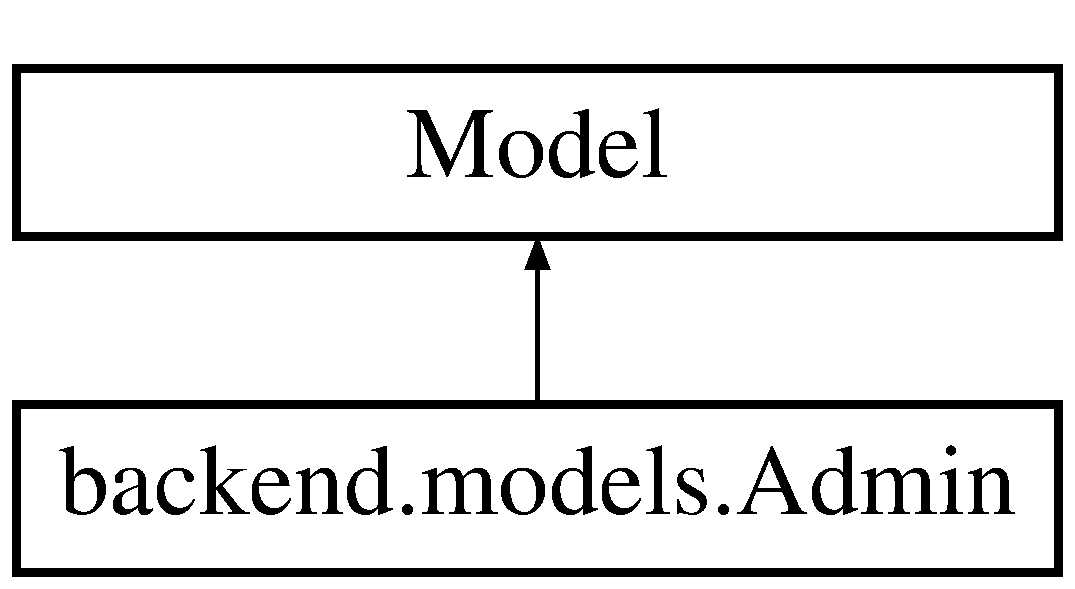
\includegraphics[height=2.000000cm]{classbackend_1_1models_1_1_admin}
\end{center}
\end{figure}
\subsection*{Static Public Attributes}
\begin{DoxyCompactItemize}
\item 
\mbox{\Hypertarget{classbackend_1_1models_1_1_admin_a9f4cd0f17f04e51e7f84370e0b8e07a6}\label{classbackend_1_1models_1_1_admin_a9f4cd0f17f04e51e7f84370e0b8e07a6}} 
{\bfseries email} = models.\+Email\+Field(default=\textquotesingle{}empty@empty.\+com\textquotesingle{}, unique=True)
\item 
\mbox{\Hypertarget{classbackend_1_1models_1_1_admin_a7d4b96d0e6b0de7e3507e20ff1a7423e}\label{classbackend_1_1models_1_1_admin_a7d4b96d0e6b0de7e3507e20ff1a7423e}} 
{\bfseries nickname} = models.\+Char\+Field(max\+\_\+length=50, default=\textquotesingle{}empty\textquotesingle{}, unique=True)
\item 
\mbox{\Hypertarget{classbackend_1_1models_1_1_admin_a92a3c7253d55521d5023e920a3912d4b}\label{classbackend_1_1models_1_1_admin_a92a3c7253d55521d5023e920a3912d4b}} 
{\bfseries password} = models.\+Char\+Field(max\+\_\+length=128, default=\textquotesingle{}empty\textquotesingle{})
\item 
\mbox{\Hypertarget{classbackend_1_1models_1_1_admin_a46af403d6c5c4b2c7f027b938dcd9d8f}\label{classbackend_1_1models_1_1_admin_a46af403d6c5c4b2c7f027b938dcd9d8f}} 
{\bfseries web\+\_\+url} = models.\+Char\+Field(max\+\_\+length=200, default=\textquotesingle{}empty\textquotesingle{}, unique=True)
\item 
\mbox{\Hypertarget{classbackend_1_1models_1_1_admin_a331198c70d1f58519956404a29051844}\label{classbackend_1_1models_1_1_admin_a331198c70d1f58519956404a29051844}} 
{\bfseries widget\+\_\+url} = models.\+Char\+Field(max\+\_\+length=200, default=\textquotesingle{}empty\textquotesingle{}, unique=True)
\item 
\mbox{\Hypertarget{classbackend_1_1models_1_1_admin_a1ba9d0e63a707f31ee02452c2b781110}\label{classbackend_1_1models_1_1_admin_a1ba9d0e63a707f31ee02452c2b781110}} 
{\bfseries mobile\+\_\+url} = models.\+Char\+Field(max\+\_\+length=200, default=\textquotesingle{}empty\textquotesingle{}, unique=True)
\item 
\mbox{\Hypertarget{classbackend_1_1models_1_1_admin_ad2c1abda1a78f6a62b010508aee974f6}\label{classbackend_1_1models_1_1_admin_ad2c1abda1a78f6a62b010508aee974f6}} 
{\bfseries communication\+\_\+key} = models.\+Char\+Field(max\+\_\+length=32, default=\textquotesingle{}empty\textquotesingle{}, unique=True)
\item 
\mbox{\Hypertarget{classbackend_1_1models_1_1_admin_a58e77c2e717073f8a19e15c150619c8f}\label{classbackend_1_1models_1_1_admin_a58e77c2e717073f8a19e15c150619c8f}} 
{\bfseries vid} = models.\+Char\+Field(max\+\_\+length=32, default=\textquotesingle{}empty\textquotesingle{})
\item 
\mbox{\Hypertarget{classbackend_1_1models_1_1_admin_aad82fd766356d3a0d7911f1076492a39}\label{classbackend_1_1models_1_1_admin_aad82fd766356d3a0d7911f1076492a39}} 
{\bfseries vid\+\_\+createtime} = models.\+Date\+Time\+Field(default=timezone.\+now, blank=True)
\end{DoxyCompactItemize}


The documentation for this class was generated from the following file\+:\begin{DoxyCompactItemize}
\item 
models.\+py\end{DoxyCompactItemize}

\hypertarget{classbackend_1_1serializers_1_1_admin_serializer}{}\section{backend.\+serializers.\+Admin\+Serializer Class Reference}
\label{classbackend_1_1serializers_1_1_admin_serializer}\index{backend.\+serializers.\+Admin\+Serializer@{backend.\+serializers.\+Admin\+Serializer}}
Inheritance diagram for backend.\+serializers.\+Admin\+Serializer\+:\begin{figure}[H]
\begin{center}
\leavevmode
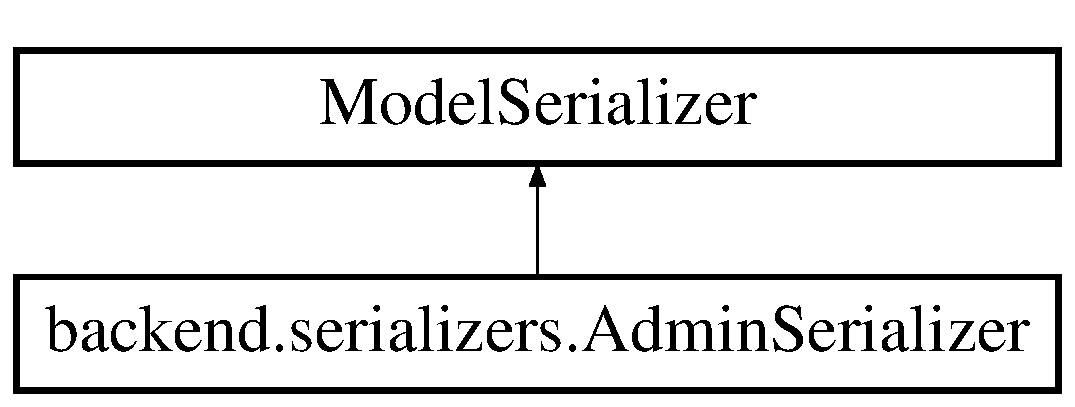
\includegraphics[height=2.000000cm]{classbackend_1_1serializers_1_1_admin_serializer}
\end{center}
\end{figure}
\subsection*{Classes}
\begin{DoxyCompactItemize}
\item 
class \hyperlink{classbackend_1_1serializers_1_1_admin_serializer_1_1_meta}{Meta}
\end{DoxyCompactItemize}


The documentation for this class was generated from the following file\+:\begin{DoxyCompactItemize}
\item 
serializers.\+py\end{DoxyCompactItemize}

\hypertarget{classbackend_1_1apps_1_1_backend_config}{}\section{backend.\+apps.\+Backend\+Config Class Reference}
\label{classbackend_1_1apps_1_1_backend_config}\index{backend.\+apps.\+Backend\+Config@{backend.\+apps.\+Backend\+Config}}
Inheritance diagram for backend.\+apps.\+Backend\+Config\+:\begin{figure}[H]
\begin{center}
\leavevmode
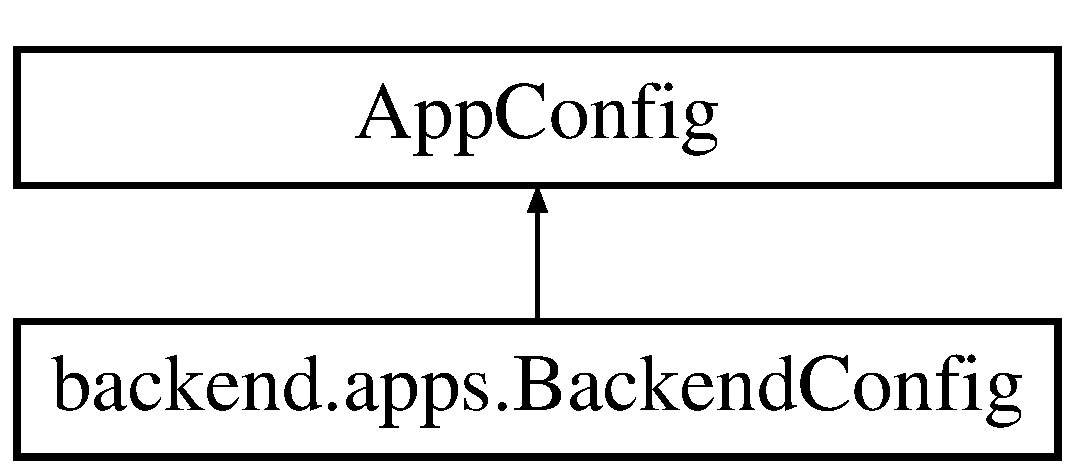
\includegraphics[height=2.000000cm]{classbackend_1_1apps_1_1_backend_config}
\end{center}
\end{figure}
\subsection*{Static Public Attributes}
\begin{DoxyCompactItemize}
\item 
\mbox{\Hypertarget{classbackend_1_1apps_1_1_backend_config_a891353e02e4b1d77f8632cf98f6f2d92}\label{classbackend_1_1apps_1_1_backend_config_a891353e02e4b1d77f8632cf98f6f2d92}} 
string {\bfseries name} = \textquotesingle{}backend\textquotesingle{}
\end{DoxyCompactItemize}


The documentation for this class was generated from the following file\+:\begin{DoxyCompactItemize}
\item 
apps.\+py\end{DoxyCompactItemize}

\hypertarget{classbackend_1_1models_1_1_big_image_log}{}\section{backend.\+models.\+Big\+Image\+Log Class Reference}
\label{classbackend_1_1models_1_1_big_image_log}\index{backend.\+models.\+Big\+Image\+Log@{backend.\+models.\+Big\+Image\+Log}}
Inheritance diagram for backend.\+models.\+Big\+Image\+Log\+:\begin{figure}[H]
\begin{center}
\leavevmode
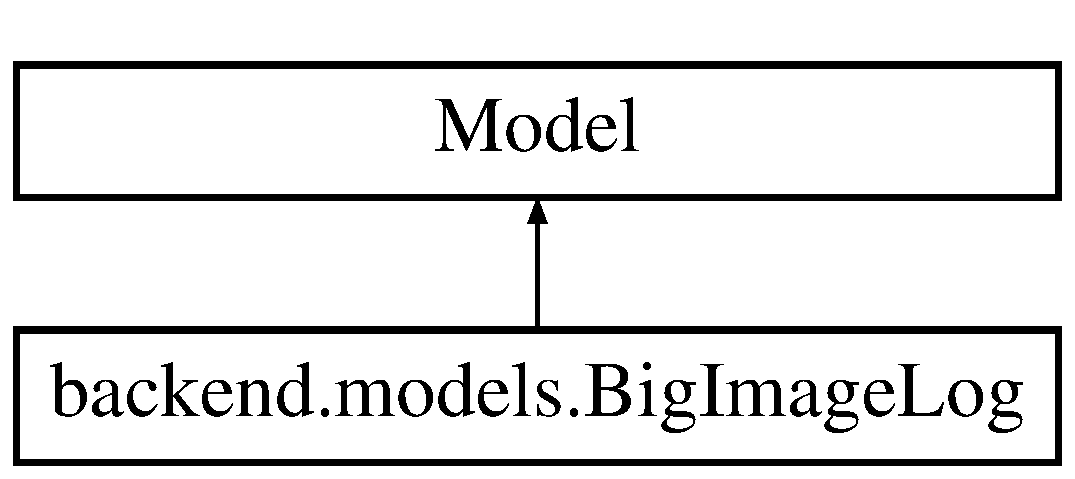
\includegraphics[height=2.000000cm]{classbackend_1_1models_1_1_big_image_log}
\end{center}
\end{figure}
\subsection*{Static Public Attributes}
\begin{DoxyCompactItemize}
\item 
\mbox{\Hypertarget{classbackend_1_1models_1_1_big_image_log_a84cf9905ea9190192e7eaa2feb32416d}\label{classbackend_1_1models_1_1_big_image_log_a84cf9905ea9190192e7eaa2feb32416d}} 
{\bfseries client\+\_\+id} = models.\+Char\+Field(max\+\_\+length=100, default=\textquotesingle{}empty\textquotesingle{})
\item 
\mbox{\Hypertarget{classbackend_1_1models_1_1_big_image_log_a63ca14bb098d823eeb1597fce63bca91}\label{classbackend_1_1models_1_1_big_image_log_a63ca14bb098d823eeb1597fce63bca91}} 
{\bfseries service\+\_\+id} = models.\+Foreign\+Key(\textquotesingle{}\hyperlink{classbackend_1_1models_1_1_customer_service}{Customer\+Service}\textquotesingle{}, on\+\_\+delete=models.\+C\+A\+S\+C\+A\+DE)
\item 
\mbox{\Hypertarget{classbackend_1_1models_1_1_big_image_log_a4535ed035d68e05dd7768a295ffc5e93}\label{classbackend_1_1models_1_1_big_image_log_a4535ed035d68e05dd7768a295ffc5e93}} 
{\bfseries image} = models.\+Image\+Field(upload\+\_\+to=\hyperlink{classbackend_1_1models__helper__functions_1_1_path_and_rename}{Path\+And\+Rename}(\textquotesingle{}user\+\_\+image/Big/\{\}\textquotesingle{}.format(time.\+strftime(\char`\"{}\%Y/\%m/\%d\char`\"{}))))
\item 
\mbox{\Hypertarget{classbackend_1_1models_1_1_big_image_log_a8f28bdaa98cdef21766ff16f4a52fedb}\label{classbackend_1_1models_1_1_big_image_log_a8f28bdaa98cdef21766ff16f4a52fedb}} 
{\bfseries extention} = models.\+Char\+Field(max\+\_\+length=10, default=\textquotesingle{}empty\textquotesingle{})
\item 
\mbox{\Hypertarget{classbackend_1_1models_1_1_big_image_log_a97e841f8fb35c4281345dc5a0cb475f2}\label{classbackend_1_1models_1_1_big_image_log_a97e841f8fb35c4281345dc5a0cb475f2}} 
{\bfseries is\+\_\+client} = models.\+Boolean\+Field(default=None)
\item 
\mbox{\Hypertarget{classbackend_1_1models_1_1_big_image_log_ad4c7330e9571492474e8c86af78e672e}\label{classbackend_1_1models_1_1_big_image_log_ad4c7330e9571492474e8c86af78e672e}} 
{\bfseries time} = models.\+Date\+Time\+Field(auto\+\_\+now\+\_\+add=True)
\item 
\mbox{\Hypertarget{classbackend_1_1models_1_1_big_image_log_ac44715f5cf49c20c3b882cbff0c6cbf1}\label{classbackend_1_1models_1_1_big_image_log_ac44715f5cf49c20c3b882cbff0c6cbf1}} 
{\bfseries label} = models.\+Char\+Field(max\+\_\+length=100, default=\textquotesingle{}empty\textquotesingle{})
\end{DoxyCompactItemize}


The documentation for this class was generated from the following file\+:\begin{DoxyCompactItemize}
\item 
models.\+py\end{DoxyCompactItemize}

\hypertarget{classbackend_1_1serializers_1_1_big_image_log_serializer}{}\section{backend.\+serializers.\+Big\+Image\+Log\+Serializer Class Reference}
\label{classbackend_1_1serializers_1_1_big_image_log_serializer}\index{backend.\+serializers.\+Big\+Image\+Log\+Serializer@{backend.\+serializers.\+Big\+Image\+Log\+Serializer}}
Inheritance diagram for backend.\+serializers.\+Big\+Image\+Log\+Serializer\+:\begin{figure}[H]
\begin{center}
\leavevmode
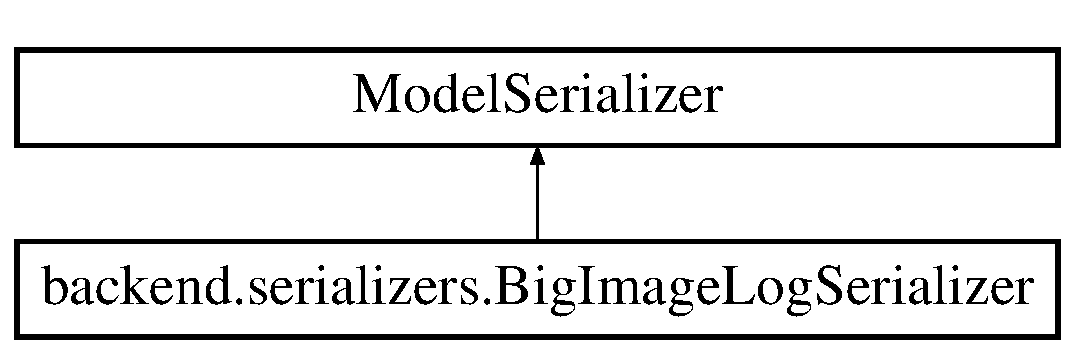
\includegraphics[height=2.000000cm]{classbackend_1_1serializers_1_1_big_image_log_serializer}
\end{center}
\end{figure}
\subsection*{Classes}
\begin{DoxyCompactItemize}
\item 
class \hyperlink{classbackend_1_1serializers_1_1_big_image_log_serializer_1_1_meta}{Meta}
\end{DoxyCompactItemize}
\subsection*{Static Public Attributes}
\begin{DoxyCompactItemize}
\item 
\mbox{\Hypertarget{classbackend_1_1serializers_1_1_big_image_log_serializer_a736735f74478b55e7378e2ba946ac110}\label{classbackend_1_1serializers_1_1_big_image_log_serializer_a736735f74478b55e7378e2ba946ac110}} 
{\bfseries image} = Base64\+Image\+Field()
\end{DoxyCompactItemize}


The documentation for this class was generated from the following file\+:\begin{DoxyCompactItemize}
\item 
serializers.\+py\end{DoxyCompactItemize}

\hypertarget{classbackend_1_1models_1_1_chatting_log}{}\section{backend.\+models.\+Chatting\+Log Class Reference}
\label{classbackend_1_1models_1_1_chatting_log}\index{backend.\+models.\+Chatting\+Log@{backend.\+models.\+Chatting\+Log}}
Inheritance diagram for backend.\+models.\+Chatting\+Log\+:\begin{figure}[H]
\begin{center}
\leavevmode
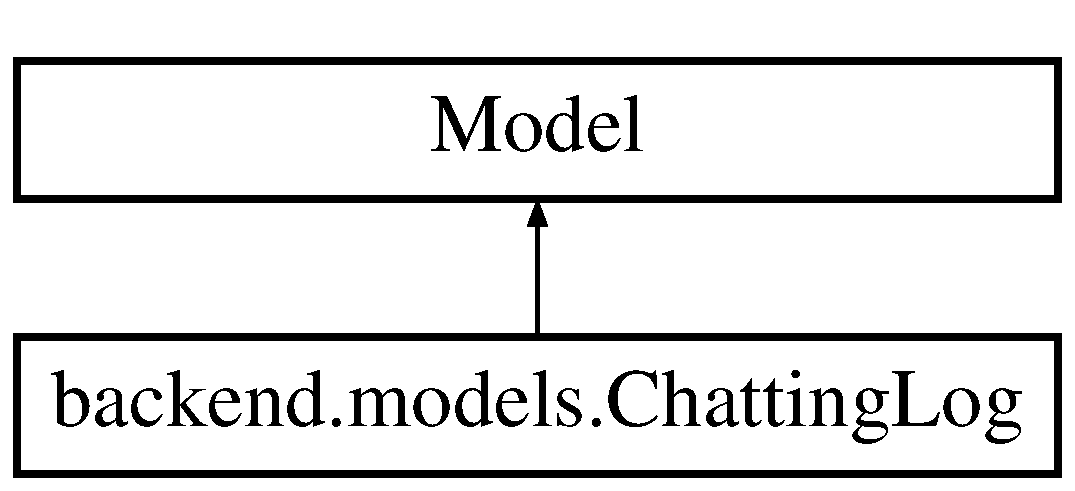
\includegraphics[height=2.000000cm]{classbackend_1_1models_1_1_chatting_log}
\end{center}
\end{figure}
\subsection*{Static Public Attributes}
\begin{DoxyCompactItemize}
\item 
\mbox{\Hypertarget{classbackend_1_1models_1_1_chatting_log_ad4a2575c5ddea616091c56a533260057}\label{classbackend_1_1models_1_1_chatting_log_ad4a2575c5ddea616091c56a533260057}} 
{\bfseries client\+\_\+id} = models.\+Char\+Field(max\+\_\+length=100, default=\textquotesingle{}empty\textquotesingle{})
\item 
\mbox{\Hypertarget{classbackend_1_1models_1_1_chatting_log_a4caf40e3ed8a77c14bed06e84a29a545}\label{classbackend_1_1models_1_1_chatting_log_a4caf40e3ed8a77c14bed06e84a29a545}} 
{\bfseries service\+\_\+id} = models.\+Foreign\+Key(\textquotesingle{}\hyperlink{classbackend_1_1models_1_1_customer_service}{Customer\+Service}\textquotesingle{}, on\+\_\+delete=models.\+C\+A\+S\+C\+A\+DE)
\item 
\mbox{\Hypertarget{classbackend_1_1models_1_1_chatting_log_a949ca36a46572fe7420dcfbd4c8405be}\label{classbackend_1_1models_1_1_chatting_log_a949ca36a46572fe7420dcfbd4c8405be}} 
{\bfseries content} = models.\+Char\+Field(max\+\_\+length=500, default=\textquotesingle{}empty\textquotesingle{})
\item 
\mbox{\Hypertarget{classbackend_1_1models_1_1_chatting_log_a9a9117e248f68e05aa590f8b0da8b9b9}\label{classbackend_1_1models_1_1_chatting_log_a9a9117e248f68e05aa590f8b0da8b9b9}} 
{\bfseries is\+\_\+client} = models.\+Boolean\+Field(default=None)
\item 
\mbox{\Hypertarget{classbackend_1_1models_1_1_chatting_log_ac521f6b7be439909cda170d4dbe5576b}\label{classbackend_1_1models_1_1_chatting_log_ac521f6b7be439909cda170d4dbe5576b}} 
{\bfseries time} = models.\+Date\+Time\+Field(auto\+\_\+now\+\_\+add=True)
\end{DoxyCompactItemize}


The documentation for this class was generated from the following file\+:\begin{DoxyCompactItemize}
\item 
models.\+py\end{DoxyCompactItemize}

\hypertarget{classbackend_1_1serializers_1_1_chatting_log_serializer}{}\section{backend.\+serializers.\+Chatting\+Log\+Serializer Class Reference}
\label{classbackend_1_1serializers_1_1_chatting_log_serializer}\index{backend.\+serializers.\+Chatting\+Log\+Serializer@{backend.\+serializers.\+Chatting\+Log\+Serializer}}
Inheritance diagram for backend.\+serializers.\+Chatting\+Log\+Serializer\+:\begin{figure}[H]
\begin{center}
\leavevmode
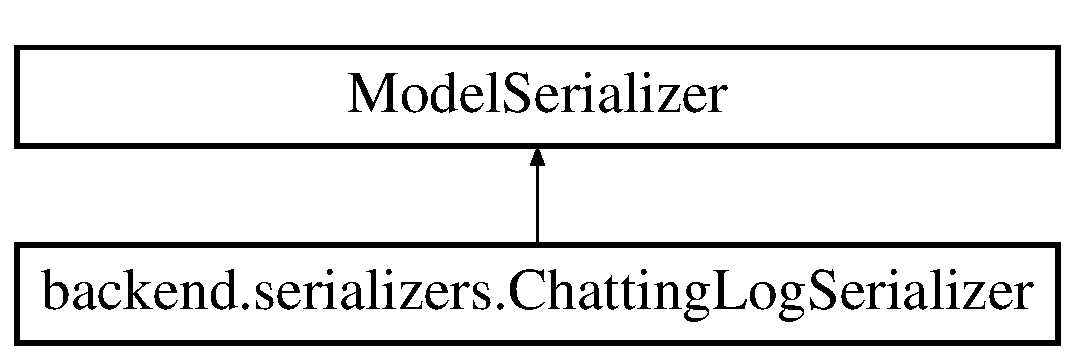
\includegraphics[height=2.000000cm]{classbackend_1_1serializers_1_1_chatting_log_serializer}
\end{center}
\end{figure}
\subsection*{Classes}
\begin{DoxyCompactItemize}
\item 
class \hyperlink{classbackend_1_1serializers_1_1_chatting_log_serializer_1_1_meta}{Meta}
\end{DoxyCompactItemize}


The documentation for this class was generated from the following file\+:\begin{DoxyCompactItemize}
\item 
serializers.\+py\end{DoxyCompactItemize}

\hypertarget{classbackend_1_1models_1_1_customer_service}{}\section{backend.\+models.\+Customer\+Service Class Reference}
\label{classbackend_1_1models_1_1_customer_service}\index{backend.\+models.\+Customer\+Service@{backend.\+models.\+Customer\+Service}}
Inheritance diagram for backend.\+models.\+Customer\+Service\+:\begin{figure}[H]
\begin{center}
\leavevmode
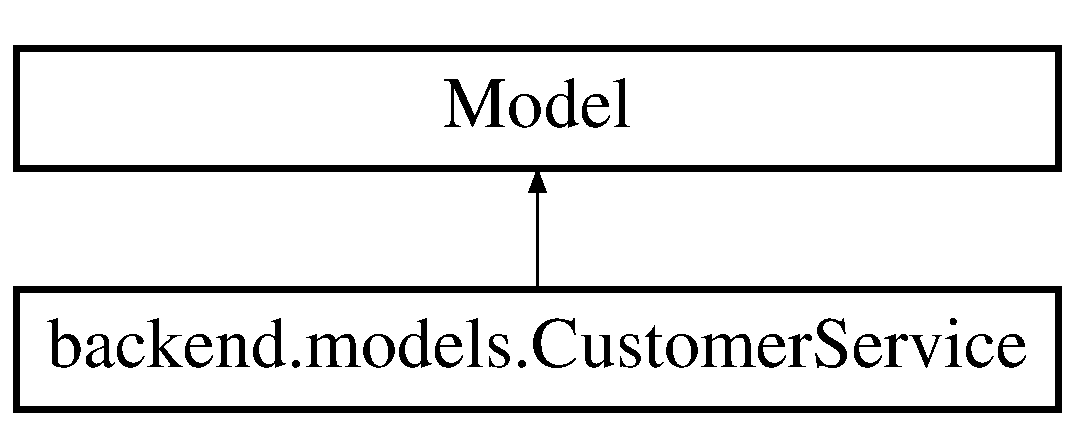
\includegraphics[height=2.000000cm]{classbackend_1_1models_1_1_customer_service}
\end{center}
\end{figure}
\subsection*{Static Public Attributes}
\begin{DoxyCompactItemize}
\item 
\mbox{\Hypertarget{classbackend_1_1models_1_1_customer_service_afd84cb13b4f13da507c1ac1d705a4a47}\label{classbackend_1_1models_1_1_customer_service_afd84cb13b4f13da507c1ac1d705a4a47}} 
{\bfseries email} = models.\+Email\+Field(default=\textquotesingle{}empty@empty.\+com\textquotesingle{}, unique=True)
\item 
\mbox{\Hypertarget{classbackend_1_1models_1_1_customer_service_a23475a354ede9af46120e17cc346da96}\label{classbackend_1_1models_1_1_customer_service_a23475a354ede9af46120e17cc346da96}} 
{\bfseries enterprise} = models.\+Foreign\+Key(\textquotesingle{}\hyperlink{classbackend_1_1models_1_1_admin}{Admin}\textquotesingle{}, on\+\_\+delete=models.\+C\+A\+S\+C\+A\+DE)
\item 
\mbox{\Hypertarget{classbackend_1_1models_1_1_customer_service_a51b7fbd597da23c46ffa48acd37a6730}\label{classbackend_1_1models_1_1_customer_service_a51b7fbd597da23c46ffa48acd37a6730}} 
{\bfseries nickname} = models.\+Char\+Field(max\+\_\+length=50, default=\textquotesingle{}empty\textquotesingle{}, unique=True)
\item 
\mbox{\Hypertarget{classbackend_1_1models_1_1_customer_service_a7aba2934fc1089c3b6730099b744debd}\label{classbackend_1_1models_1_1_customer_service_a7aba2934fc1089c3b6730099b744debd}} 
{\bfseries password} = models.\+Char\+Field(max\+\_\+length=128, default=\textquotesingle{}empty\textquotesingle{})
\item 
\mbox{\Hypertarget{classbackend_1_1models_1_1_customer_service_a316a7ce100879a6fb27a8d202a857ab9}\label{classbackend_1_1models_1_1_customer_service_a316a7ce100879a6fb27a8d202a857ab9}} 
{\bfseries is\+\_\+register} = models.\+Boolean\+Field(default=False)
\item 
\mbox{\Hypertarget{classbackend_1_1models_1_1_customer_service_a35d1452178e9d8ce83e0abaebbcfa060}\label{classbackend_1_1models_1_1_customer_service_a35d1452178e9d8ce83e0abaebbcfa060}} 
{\bfseries is\+\_\+online} = models.\+Boolean\+Field(default=False)
\item 
\mbox{\Hypertarget{classbackend_1_1models_1_1_customer_service_a2ac1c6d11ccc775f4a8c40ddd436967d}\label{classbackend_1_1models_1_1_customer_service_a2ac1c6d11ccc775f4a8c40ddd436967d}} 
{\bfseries connection\+\_\+num} = models.\+Integer\+Field(default=0)
\item 
\mbox{\Hypertarget{classbackend_1_1models_1_1_customer_service_afed4ee03d4fddfda167fd0970f369488}\label{classbackend_1_1models_1_1_customer_service_afed4ee03d4fddfda167fd0970f369488}} 
{\bfseries vid} = models.\+Char\+Field(max\+\_\+length=32, default=\textquotesingle{}empty\textquotesingle{})
\item 
\mbox{\Hypertarget{classbackend_1_1models_1_1_customer_service_ad6e0221ddd7b485e04f156e3eb935c31}\label{classbackend_1_1models_1_1_customer_service_ad6e0221ddd7b485e04f156e3eb935c31}} 
{\bfseries vid\+\_\+createtime} = models.\+Date\+Time\+Field(default=timezone.\+now, blank=True)
\end{DoxyCompactItemize}


The documentation for this class was generated from the following file\+:\begin{DoxyCompactItemize}
\item 
models.\+py\end{DoxyCompactItemize}

\hypertarget{classbackend_1_1serializers_1_1_customer_service_create_serializer}{}\section{backend.\+serializers.\+Customer\+Service\+Create\+Serializer Class Reference}
\label{classbackend_1_1serializers_1_1_customer_service_create_serializer}\index{backend.\+serializers.\+Customer\+Service\+Create\+Serializer@{backend.\+serializers.\+Customer\+Service\+Create\+Serializer}}
Inheritance diagram for backend.\+serializers.\+Customer\+Service\+Create\+Serializer\+:\begin{figure}[H]
\begin{center}
\leavevmode
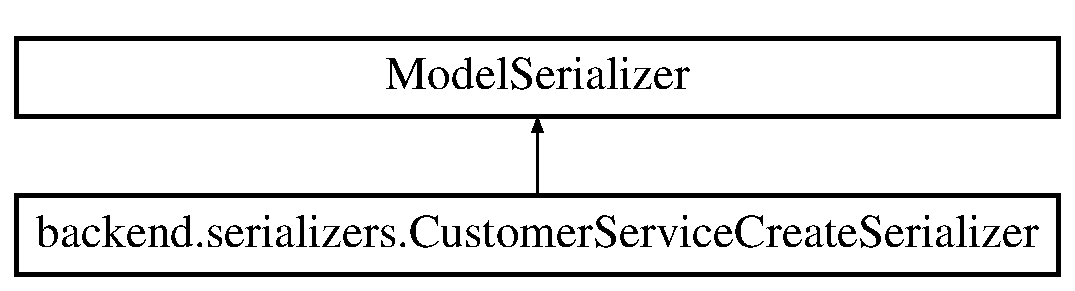
\includegraphics[height=2.000000cm]{classbackend_1_1serializers_1_1_customer_service_create_serializer}
\end{center}
\end{figure}
\subsection*{Classes}
\begin{DoxyCompactItemize}
\item 
class \hyperlink{classbackend_1_1serializers_1_1_customer_service_create_serializer_1_1_meta}{Meta}
\end{DoxyCompactItemize}


The documentation for this class was generated from the following file\+:\begin{DoxyCompactItemize}
\item 
serializers.\+py\end{DoxyCompactItemize}

\hypertarget{classbackend_1_1serializers_1_1_customer_service_serializer}{}\section{backend.\+serializers.\+Customer\+Service\+Serializer Class Reference}
\label{classbackend_1_1serializers_1_1_customer_service_serializer}\index{backend.\+serializers.\+Customer\+Service\+Serializer@{backend.\+serializers.\+Customer\+Service\+Serializer}}
Inheritance diagram for backend.\+serializers.\+Customer\+Service\+Serializer\+:\begin{figure}[H]
\begin{center}
\leavevmode
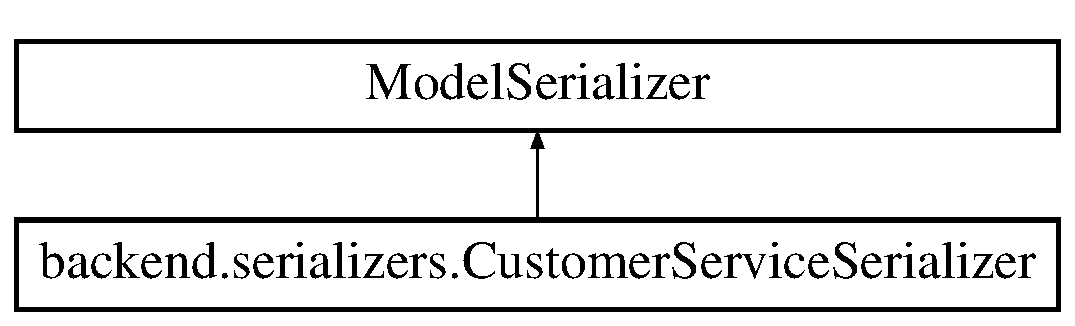
\includegraphics[height=2.000000cm]{classbackend_1_1serializers_1_1_customer_service_serializer}
\end{center}
\end{figure}
\subsection*{Classes}
\begin{DoxyCompactItemize}
\item 
class \hyperlink{classbackend_1_1serializers_1_1_customer_service_serializer_1_1_meta}{Meta}
\end{DoxyCompactItemize}


The documentation for this class was generated from the following file\+:\begin{DoxyCompactItemize}
\item 
serializers.\+py\end{DoxyCompactItemize}

\hypertarget{classbackend_1_1models_1_1_enterprise_display_info}{}\section{backend.\+models.\+Enterprise\+Display\+Info Class Reference}
\label{classbackend_1_1models_1_1_enterprise_display_info}\index{backend.\+models.\+Enterprise\+Display\+Info@{backend.\+models.\+Enterprise\+Display\+Info}}
Inheritance diagram for backend.\+models.\+Enterprise\+Display\+Info\+:\begin{figure}[H]
\begin{center}
\leavevmode
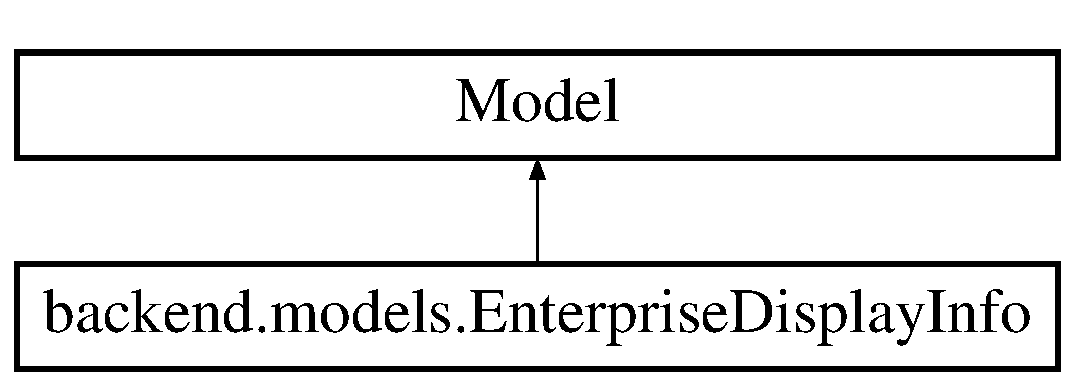
\includegraphics[height=2.000000cm]{classbackend_1_1models_1_1_enterprise_display_info}
\end{center}
\end{figure}
\subsection*{Static Public Attributes}
\begin{DoxyCompactItemize}
\item 
\mbox{\Hypertarget{classbackend_1_1models_1_1_enterprise_display_info_a9ea91f67e8567166cddc5ec8732faaf5}\label{classbackend_1_1models_1_1_enterprise_display_info_a9ea91f67e8567166cddc5ec8732faaf5}} 
{\bfseries enterprise} = models.\+Foreign\+Key(\textquotesingle{}\hyperlink{classbackend_1_1models_1_1_admin}{Admin}\textquotesingle{}, on\+\_\+delete=models.\+C\+A\+S\+C\+A\+DE)
\item 
\mbox{\Hypertarget{classbackend_1_1models_1_1_enterprise_display_info_a6940007546968826af9eadc523c6c9cc}\label{classbackend_1_1models_1_1_enterprise_display_info_a6940007546968826af9eadc523c6c9cc}} 
{\bfseries name} = models.\+Char\+Field(max\+\_\+length=50, default=\textquotesingle{}empty\textquotesingle{})
\item 
\mbox{\Hypertarget{classbackend_1_1models_1_1_enterprise_display_info_a1e0f27692b566dcb1dda1d9ae087fd41}\label{classbackend_1_1models_1_1_enterprise_display_info_a1e0f27692b566dcb1dda1d9ae087fd41}} 
{\bfseries comment} = models.\+Char\+Field(max\+\_\+length=200, default=\textquotesingle{}\textquotesingle{}, blank=True)
\end{DoxyCompactItemize}


The documentation for this class was generated from the following file\+:\begin{DoxyCompactItemize}
\item 
models.\+py\end{DoxyCompactItemize}

\hypertarget{classbackend_1_1serializers_1_1_enterprise_display_info_serializer}{}\section{backend.\+serializers.\+Enterprise\+Display\+Info\+Serializer Class Reference}
\label{classbackend_1_1serializers_1_1_enterprise_display_info_serializer}\index{backend.\+serializers.\+Enterprise\+Display\+Info\+Serializer@{backend.\+serializers.\+Enterprise\+Display\+Info\+Serializer}}
Inheritance diagram for backend.\+serializers.\+Enterprise\+Display\+Info\+Serializer\+:\begin{figure}[H]
\begin{center}
\leavevmode
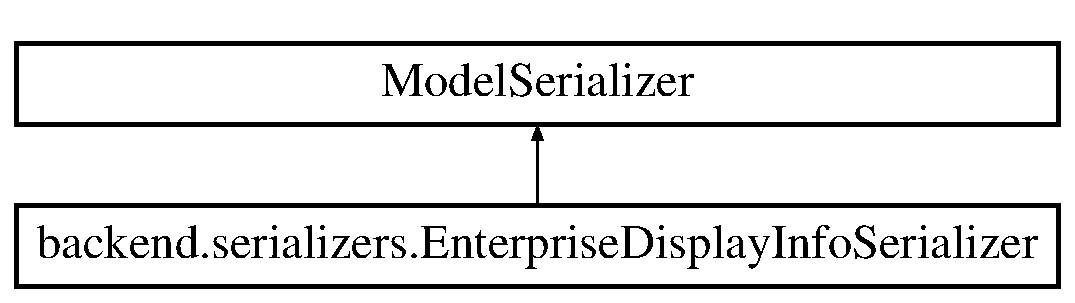
\includegraphics[height=2.000000cm]{classbackend_1_1serializers_1_1_enterprise_display_info_serializer}
\end{center}
\end{figure}
\subsection*{Classes}
\begin{DoxyCompactItemize}
\item 
class \hyperlink{classbackend_1_1serializers_1_1_enterprise_display_info_serializer_1_1_meta}{Meta}
\end{DoxyCompactItemize}


The documentation for this class was generated from the following file\+:\begin{DoxyCompactItemize}
\item 
serializers.\+py\end{DoxyCompactItemize}

\hypertarget{classbackend_1_1serializers_1_1_enterprise_display_info_serializer_1_1_meta}{}\section{backend.\+serializers.\+Enterprise\+Display\+Info\+Serializer.\+Meta Class Reference}
\label{classbackend_1_1serializers_1_1_enterprise_display_info_serializer_1_1_meta}\index{backend.\+serializers.\+Enterprise\+Display\+Info\+Serializer.\+Meta@{backend.\+serializers.\+Enterprise\+Display\+Info\+Serializer.\+Meta}}
\subsection*{Static Public Attributes}
\begin{DoxyCompactItemize}
\item 
\mbox{\Hypertarget{classbackend_1_1serializers_1_1_enterprise_display_info_serializer_1_1_meta_ad352130f940b5756dd8c2262d77ce747}\label{classbackend_1_1serializers_1_1_enterprise_display_info_serializer_1_1_meta_ad352130f940b5756dd8c2262d77ce747}} 
{\bfseries model} = \hyperlink{classbackend_1_1models_1_1_enterprise_display_info}{Enterprise\+Display\+Info}
\item 
\mbox{\Hypertarget{classbackend_1_1serializers_1_1_enterprise_display_info_serializer_1_1_meta_ac0c98b8da43b375efb0a4321079d7c95}\label{classbackend_1_1serializers_1_1_enterprise_display_info_serializer_1_1_meta_ac0c98b8da43b375efb0a4321079d7c95}} 
tuple {\bfseries fields} = (\textquotesingle{}id\textquotesingle{}, \textquotesingle{}enterprise\textquotesingle{}, \textquotesingle{}name\textquotesingle{}, \textquotesingle{}comment\textquotesingle{})
\end{DoxyCompactItemize}


The documentation for this class was generated from the following file\+:\begin{DoxyCompactItemize}
\item 
serializers.\+py\end{DoxyCompactItemize}

\hypertarget{classbackend_1_1serializers_1_1_customer_service_serializer_1_1_meta}{}\section{backend.\+serializers.\+Customer\+Service\+Serializer.\+Meta Class Reference}
\label{classbackend_1_1serializers_1_1_customer_service_serializer_1_1_meta}\index{backend.\+serializers.\+Customer\+Service\+Serializer.\+Meta@{backend.\+serializers.\+Customer\+Service\+Serializer.\+Meta}}
\subsection*{Static Public Attributes}
\begin{DoxyCompactItemize}
\item 
\mbox{\Hypertarget{classbackend_1_1serializers_1_1_customer_service_serializer_1_1_meta_a37c677b65630698219d4783021068c22}\label{classbackend_1_1serializers_1_1_customer_service_serializer_1_1_meta_a37c677b65630698219d4783021068c22}} 
{\bfseries model} = \hyperlink{classbackend_1_1models_1_1_customer_service}{Customer\+Service}
\item 
\mbox{\Hypertarget{classbackend_1_1serializers_1_1_customer_service_serializer_1_1_meta_a136971cbeacbcde4b66040534539ed35}\label{classbackend_1_1serializers_1_1_customer_service_serializer_1_1_meta_a136971cbeacbcde4b66040534539ed35}} 
tuple {\bfseries fields} = (\textquotesingle{}id\textquotesingle{}, \textquotesingle{}email\textquotesingle{}, \textquotesingle{}nickname\textquotesingle{}, \textquotesingle{}password\textquotesingle{}, \textquotesingle{}is\+\_\+register\textquotesingle{}, \textquotesingle{}is\+\_\+online\textquotesingle{}, \textquotesingle{}connection\+\_\+num\textquotesingle{}, \textquotesingle{}vid\textquotesingle{}, \textquotesingle{}vid\+\_\+createtime\textquotesingle{})
\end{DoxyCompactItemize}


The documentation for this class was generated from the following file\+:\begin{DoxyCompactItemize}
\item 
serializers.\+py\end{DoxyCompactItemize}

\hypertarget{classbackend_1_1serializers_1_1_chatting_log_serializer_1_1_meta}{}\section{backend.\+serializers.\+Chatting\+Log\+Serializer.\+Meta Class Reference}
\label{classbackend_1_1serializers_1_1_chatting_log_serializer_1_1_meta}\index{backend.\+serializers.\+Chatting\+Log\+Serializer.\+Meta@{backend.\+serializers.\+Chatting\+Log\+Serializer.\+Meta}}
\subsection*{Static Public Attributes}
\begin{DoxyCompactItemize}
\item 
\mbox{\Hypertarget{classbackend_1_1serializers_1_1_chatting_log_serializer_1_1_meta_ad9ece68b9b4417b89153704421118635}\label{classbackend_1_1serializers_1_1_chatting_log_serializer_1_1_meta_ad9ece68b9b4417b89153704421118635}} 
{\bfseries model} = \hyperlink{classbackend_1_1models_1_1_chatting_log}{Chatting\+Log}
\item 
\mbox{\Hypertarget{classbackend_1_1serializers_1_1_chatting_log_serializer_1_1_meta_aa11cd94675f54272c4541b62bc715300}\label{classbackend_1_1serializers_1_1_chatting_log_serializer_1_1_meta_aa11cd94675f54272c4541b62bc715300}} 
tuple {\bfseries fields} = (\textquotesingle{}id\textquotesingle{}, \textquotesingle{}client\+\_\+id\textquotesingle{}, \textquotesingle{}service\+\_\+id\textquotesingle{}, \textquotesingle{}content\textquotesingle{}, \textquotesingle{}is\+\_\+client\textquotesingle{}, \textquotesingle{}time\textquotesingle{})
\end{DoxyCompactItemize}


The documentation for this class was generated from the following file\+:\begin{DoxyCompactItemize}
\item 
serializers.\+py\end{DoxyCompactItemize}

\hypertarget{classbackend_1_1serializers_1_1_serial_number_serializer_1_1_meta}{}\section{backend.\+serializers.\+Serial\+Number\+Serializer.\+Meta Class Reference}
\label{classbackend_1_1serializers_1_1_serial_number_serializer_1_1_meta}\index{backend.\+serializers.\+Serial\+Number\+Serializer.\+Meta@{backend.\+serializers.\+Serial\+Number\+Serializer.\+Meta}}
\subsection*{Static Public Attributes}
\begin{DoxyCompactItemize}
\item 
\mbox{\Hypertarget{classbackend_1_1serializers_1_1_serial_number_serializer_1_1_meta_a10bd241c79ff0b305cb5ab32927fbafa}\label{classbackend_1_1serializers_1_1_serial_number_serializer_1_1_meta_a10bd241c79ff0b305cb5ab32927fbafa}} 
{\bfseries model} = \hyperlink{classbackend_1_1models_1_1_serial_number}{Serial\+Number}
\item 
\mbox{\Hypertarget{classbackend_1_1serializers_1_1_serial_number_serializer_1_1_meta_aa0c41685a36666a77fb4411e6c840c33}\label{classbackend_1_1serializers_1_1_serial_number_serializer_1_1_meta_aa0c41685a36666a77fb4411e6c840c33}} 
tuple {\bfseries fields} = (\textquotesingle{}id\textquotesingle{}, \textquotesingle{}serials\textquotesingle{}, \textquotesingle{}is\+\_\+used\textquotesingle{})
\end{DoxyCompactItemize}


The documentation for this class was generated from the following file\+:\begin{DoxyCompactItemize}
\item 
serializers.\+py\end{DoxyCompactItemize}

\hypertarget{classbackend_1_1serializers_1_1_big_image_log_serializer_1_1_meta}{}\section{backend.\+serializers.\+Big\+Image\+Log\+Serializer.\+Meta Class Reference}
\label{classbackend_1_1serializers_1_1_big_image_log_serializer_1_1_meta}\index{backend.\+serializers.\+Big\+Image\+Log\+Serializer.\+Meta@{backend.\+serializers.\+Big\+Image\+Log\+Serializer.\+Meta}}
\subsection*{Static Public Attributes}
\begin{DoxyCompactItemize}
\item 
\mbox{\Hypertarget{classbackend_1_1serializers_1_1_big_image_log_serializer_1_1_meta_a681235c1c088390e50d25550342e5026}\label{classbackend_1_1serializers_1_1_big_image_log_serializer_1_1_meta_a681235c1c088390e50d25550342e5026}} 
{\bfseries model} = \hyperlink{classbackend_1_1models_1_1_big_image_log}{Big\+Image\+Log}
\item 
\mbox{\Hypertarget{classbackend_1_1serializers_1_1_big_image_log_serializer_1_1_meta_a1def8357c9828f7b4237cd81de01c908}\label{classbackend_1_1serializers_1_1_big_image_log_serializer_1_1_meta_a1def8357c9828f7b4237cd81de01c908}} 
tuple {\bfseries fields} = (\textquotesingle{}id\textquotesingle{}, \textquotesingle{}client\+\_\+id\textquotesingle{}, \textquotesingle{}service\+\_\+id\textquotesingle{}, \textquotesingle{}image\textquotesingle{}, \textquotesingle{}extention\textquotesingle{}, \textquotesingle{}is\+\_\+client\textquotesingle{}, \textquotesingle{}time\textquotesingle{}, \textquotesingle{}label\textquotesingle{})
\end{DoxyCompactItemize}


The documentation for this class was generated from the following file\+:\begin{DoxyCompactItemize}
\item 
serializers.\+py\end{DoxyCompactItemize}

\hypertarget{classbackend_1_1serializers_1_1_small_image_log_serializer_1_1_meta}{}\section{backend.\+serializers.\+Small\+Image\+Log\+Serializer.\+Meta Class Reference}
\label{classbackend_1_1serializers_1_1_small_image_log_serializer_1_1_meta}\index{backend.\+serializers.\+Small\+Image\+Log\+Serializer.\+Meta@{backend.\+serializers.\+Small\+Image\+Log\+Serializer.\+Meta}}
\subsection*{Static Public Attributes}
\begin{DoxyCompactItemize}
\item 
\mbox{\Hypertarget{classbackend_1_1serializers_1_1_small_image_log_serializer_1_1_meta_a621764f37d90f62beaa2c9da8caaf26b}\label{classbackend_1_1serializers_1_1_small_image_log_serializer_1_1_meta_a621764f37d90f62beaa2c9da8caaf26b}} 
{\bfseries model} = \hyperlink{classbackend_1_1models_1_1_small_image_log}{Small\+Image\+Log}
\item 
\mbox{\Hypertarget{classbackend_1_1serializers_1_1_small_image_log_serializer_1_1_meta_a772311e5544e3426c23c18a7e1a85074}\label{classbackend_1_1serializers_1_1_small_image_log_serializer_1_1_meta_a772311e5544e3426c23c18a7e1a85074}} 
tuple {\bfseries fields} = (\textquotesingle{}id\textquotesingle{}, \textquotesingle{}client\+\_\+id\textquotesingle{}, \textquotesingle{}service\+\_\+id\textquotesingle{}, \textquotesingle{}image\textquotesingle{}, \textquotesingle{}extention\textquotesingle{}, \textquotesingle{}is\+\_\+client\textquotesingle{}, \textquotesingle{}time\textquotesingle{}, \textquotesingle{}label\textquotesingle{})
\end{DoxyCompactItemize}


The documentation for this class was generated from the following file\+:\begin{DoxyCompactItemize}
\item 
serializers.\+py\end{DoxyCompactItemize}

\hypertarget{classbackend_1_1serializers_1_1_customer_service_create_serializer_1_1_meta}{}\section{backend.\+serializers.\+Customer\+Service\+Create\+Serializer.\+Meta Class Reference}
\label{classbackend_1_1serializers_1_1_customer_service_create_serializer_1_1_meta}\index{backend.\+serializers.\+Customer\+Service\+Create\+Serializer.\+Meta@{backend.\+serializers.\+Customer\+Service\+Create\+Serializer.\+Meta}}
\subsection*{Static Public Attributes}
\begin{DoxyCompactItemize}
\item 
\mbox{\Hypertarget{classbackend_1_1serializers_1_1_customer_service_create_serializer_1_1_meta_ab1c442911fd2fd8df0d6b7ffb286318c}\label{classbackend_1_1serializers_1_1_customer_service_create_serializer_1_1_meta_ab1c442911fd2fd8df0d6b7ffb286318c}} 
{\bfseries model} = \hyperlink{classbackend_1_1models_1_1_customer_service}{Customer\+Service}
\item 
\mbox{\Hypertarget{classbackend_1_1serializers_1_1_customer_service_create_serializer_1_1_meta_aae59f21e55a2452eb316500ded264b6a}\label{classbackend_1_1serializers_1_1_customer_service_create_serializer_1_1_meta_aae59f21e55a2452eb316500ded264b6a}} 
tuple {\bfseries fields} = (\textquotesingle{}id\textquotesingle{}, \textquotesingle{}email\textquotesingle{}, \textquotesingle{}enterprise\textquotesingle{}, \textquotesingle{}nickname\textquotesingle{}, \textquotesingle{}password\textquotesingle{}, \textquotesingle{}is\+\_\+register\textquotesingle{}, \textquotesingle{}is\+\_\+online\textquotesingle{}, \textquotesingle{}connection\+\_\+num\textquotesingle{}, \textquotesingle{}vid\textquotesingle{}, \textquotesingle{}vid\+\_\+createtime\textquotesingle{})
\end{DoxyCompactItemize}


The documentation for this class was generated from the following file\+:\begin{DoxyCompactItemize}
\item 
serializers.\+py\end{DoxyCompactItemize}

\hypertarget{classbackend_1_1serializers_1_1_admin_serializer_1_1_meta}{}\section{backend.\+serializers.\+Admin\+Serializer.\+Meta Class Reference}
\label{classbackend_1_1serializers_1_1_admin_serializer_1_1_meta}\index{backend.\+serializers.\+Admin\+Serializer.\+Meta@{backend.\+serializers.\+Admin\+Serializer.\+Meta}}
\subsection*{Static Public Attributes}
\begin{DoxyCompactItemize}
\item 
\mbox{\Hypertarget{classbackend_1_1serializers_1_1_admin_serializer_1_1_meta_a78d97ca03730721da56aab4c49f8d13c}\label{classbackend_1_1serializers_1_1_admin_serializer_1_1_meta_a78d97ca03730721da56aab4c49f8d13c}} 
{\bfseries model} = \hyperlink{classbackend_1_1models_1_1_admin}{Admin}
\item 
\mbox{\Hypertarget{classbackend_1_1serializers_1_1_admin_serializer_1_1_meta_a74859ad8304c06766af6e1819ab4c63f}\label{classbackend_1_1serializers_1_1_admin_serializer_1_1_meta_a74859ad8304c06766af6e1819ab4c63f}} 
tuple {\bfseries fields} = (\textquotesingle{}id\textquotesingle{}, \textquotesingle{}email\textquotesingle{}, \textquotesingle{}nickname\textquotesingle{}, \textquotesingle{}password\textquotesingle{}, \textquotesingle{}web\+\_\+url\textquotesingle{}, \textquotesingle{}widget\+\_\+url\textquotesingle{}, \textquotesingle{}mobile\+\_\+url\textquotesingle{}, \textquotesingle{}communication\+\_\+key\textquotesingle{}, \textquotesingle{}vid\textquotesingle{}, \textquotesingle{}vid\+\_\+createtime\textquotesingle{})
\end{DoxyCompactItemize}


The documentation for this class was generated from the following file\+:\begin{DoxyCompactItemize}
\item 
serializers.\+py\end{DoxyCompactItemize}

\hypertarget{classbackend_1_1serializers_1_1_robot_info_serializer_1_1_meta}{}\section{backend.\+serializers.\+Robot\+Info\+Serializer.\+Meta Class Reference}
\label{classbackend_1_1serializers_1_1_robot_info_serializer_1_1_meta}\index{backend.\+serializers.\+Robot\+Info\+Serializer.\+Meta@{backend.\+serializers.\+Robot\+Info\+Serializer.\+Meta}}
\subsection*{Static Public Attributes}
\begin{DoxyCompactItemize}
\item 
\mbox{\Hypertarget{classbackend_1_1serializers_1_1_robot_info_serializer_1_1_meta_a9e28194531554ddadda68a8739c2513c}\label{classbackend_1_1serializers_1_1_robot_info_serializer_1_1_meta_a9e28194531554ddadda68a8739c2513c}} 
{\bfseries model} = \hyperlink{classbackend_1_1models_1_1_robot_info}{Robot\+Info}
\item 
\mbox{\Hypertarget{classbackend_1_1serializers_1_1_robot_info_serializer_1_1_meta_a50657ceec4d129050450190a7dc9e5f9}\label{classbackend_1_1serializers_1_1_robot_info_serializer_1_1_meta_a50657ceec4d129050450190a7dc9e5f9}} 
tuple {\bfseries fields} = (\textquotesingle{}id\textquotesingle{}, \textquotesingle{}enterprise\textquotesingle{}, \textquotesingle{}question\textquotesingle{}, \textquotesingle{}answer\textquotesingle{}, \textquotesingle{}keyword\textquotesingle{}, \textquotesingle{}weight\textquotesingle{})
\end{DoxyCompactItemize}


The documentation for this class was generated from the following file\+:\begin{DoxyCompactItemize}
\item 
serializers.\+py\end{DoxyCompactItemize}

\hypertarget{classbackend_1_1models__helper__functions_1_1_path_and_rename}{}\section{backend.\+models\+\_\+helper\+\_\+functions.\+Path\+And\+Rename Class Reference}
\label{classbackend_1_1models__helper__functions_1_1_path_and_rename}\index{backend.\+models\+\_\+helper\+\_\+functions.\+Path\+And\+Rename@{backend.\+models\+\_\+helper\+\_\+functions.\+Path\+And\+Rename}}
Inheritance diagram for backend.\+models\+\_\+helper\+\_\+functions.\+Path\+And\+Rename\+:\begin{figure}[H]
\begin{center}
\leavevmode
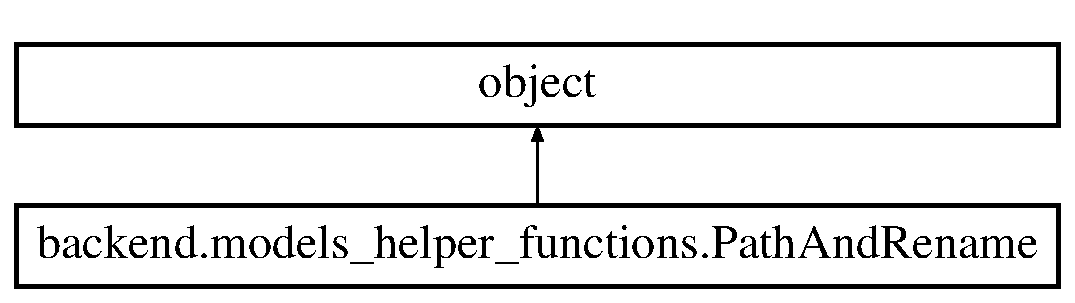
\includegraphics[height=2.000000cm]{classbackend_1_1models__helper__functions_1_1_path_and_rename}
\end{center}
\end{figure}
\subsection*{Public Member Functions}
\begin{DoxyCompactItemize}
\item 
\mbox{\Hypertarget{classbackend_1_1models__helper__functions_1_1_path_and_rename_aded3c71835bd5d6a1fe6d55adf4491fe}\label{classbackend_1_1models__helper__functions_1_1_path_and_rename_aded3c71835bd5d6a1fe6d55adf4491fe}} 
def {\bfseries \+\_\+\+\_\+init\+\_\+\+\_\+} (self, sub\+\_\+path)
\item 
\mbox{\Hypertarget{classbackend_1_1models__helper__functions_1_1_path_and_rename_a7f6788b9fb77beb7a91c6b180214f8a1}\label{classbackend_1_1models__helper__functions_1_1_path_and_rename_a7f6788b9fb77beb7a91c6b180214f8a1}} 
def {\bfseries \+\_\+\+\_\+call\+\_\+\+\_\+} (self, instance, filename)
\end{DoxyCompactItemize}
\subsection*{Public Attributes}
\begin{DoxyCompactItemize}
\item 
\mbox{\Hypertarget{classbackend_1_1models__helper__functions_1_1_path_and_rename_aff2db7313bc72e1038fd13187c057883}\label{classbackend_1_1models__helper__functions_1_1_path_and_rename_aff2db7313bc72e1038fd13187c057883}} 
{\bfseries path}
\end{DoxyCompactItemize}


The documentation for this class was generated from the following file\+:\begin{DoxyCompactItemize}
\item 
models\+\_\+helper\+\_\+functions.\+py\end{DoxyCompactItemize}

\hypertarget{classbackend_1_1models_1_1_robot_gossip_info}{}\section{backend.\+models.\+Robot\+Gossip\+Info Class Reference}
\label{classbackend_1_1models_1_1_robot_gossip_info}\index{backend.\+models.\+Robot\+Gossip\+Info@{backend.\+models.\+Robot\+Gossip\+Info}}
Inheritance diagram for backend.\+models.\+Robot\+Gossip\+Info\+:\begin{figure}[H]
\begin{center}
\leavevmode
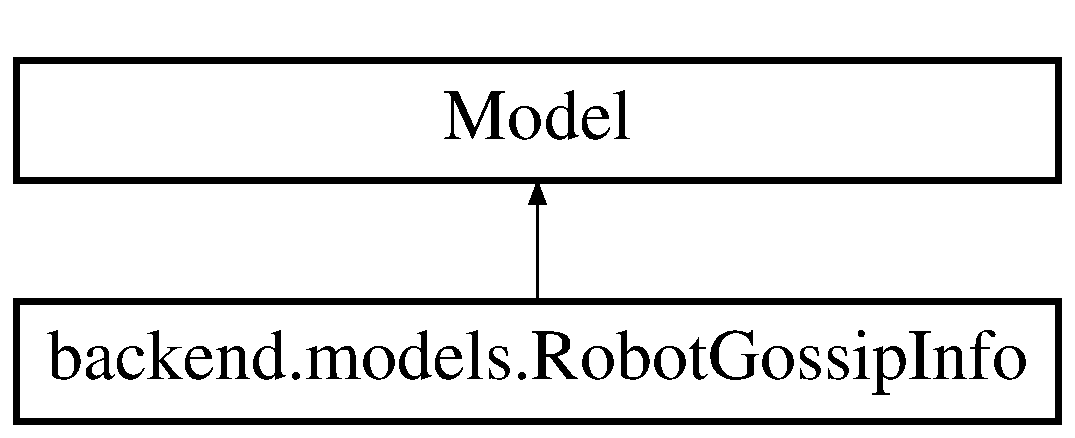
\includegraphics[height=2.000000cm]{classbackend_1_1models_1_1_robot_gossip_info}
\end{center}
\end{figure}
\subsection*{Static Public Attributes}
\begin{DoxyCompactItemize}
\item 
\mbox{\Hypertarget{classbackend_1_1models_1_1_robot_gossip_info_a90210f78f32779caed97c97ae01dac60}\label{classbackend_1_1models_1_1_robot_gossip_info_a90210f78f32779caed97c97ae01dac60}} 
{\bfseries question} = models.\+Char\+Field(max\+\_\+length=150, default=\textquotesingle{}empty\textquotesingle{})
\item 
\mbox{\Hypertarget{classbackend_1_1models_1_1_robot_gossip_info_adc77a4dc8003d7a4aee99da89b73d5b3}\label{classbackend_1_1models_1_1_robot_gossip_info_adc77a4dc8003d7a4aee99da89b73d5b3}} 
{\bfseries answer} = models.\+Char\+Field(max\+\_\+length=500, default=\textquotesingle{}empty\textquotesingle{})
\item 
\mbox{\Hypertarget{classbackend_1_1models_1_1_robot_gossip_info_add18723982e6c3272edb001c841c7ca1}\label{classbackend_1_1models_1_1_robot_gossip_info_add18723982e6c3272edb001c841c7ca1}} 
{\bfseries weight} = models.\+Integer\+Field(default=1)
\end{DoxyCompactItemize}


The documentation for this class was generated from the following file\+:\begin{DoxyCompactItemize}
\item 
models.\+py\end{DoxyCompactItemize}

\hypertarget{classbackend_1_1models_1_1_robot_info}{}\section{backend.\+models.\+Robot\+Info Class Reference}
\label{classbackend_1_1models_1_1_robot_info}\index{backend.\+models.\+Robot\+Info@{backend.\+models.\+Robot\+Info}}
Inheritance diagram for backend.\+models.\+Robot\+Info\+:\begin{figure}[H]
\begin{center}
\leavevmode
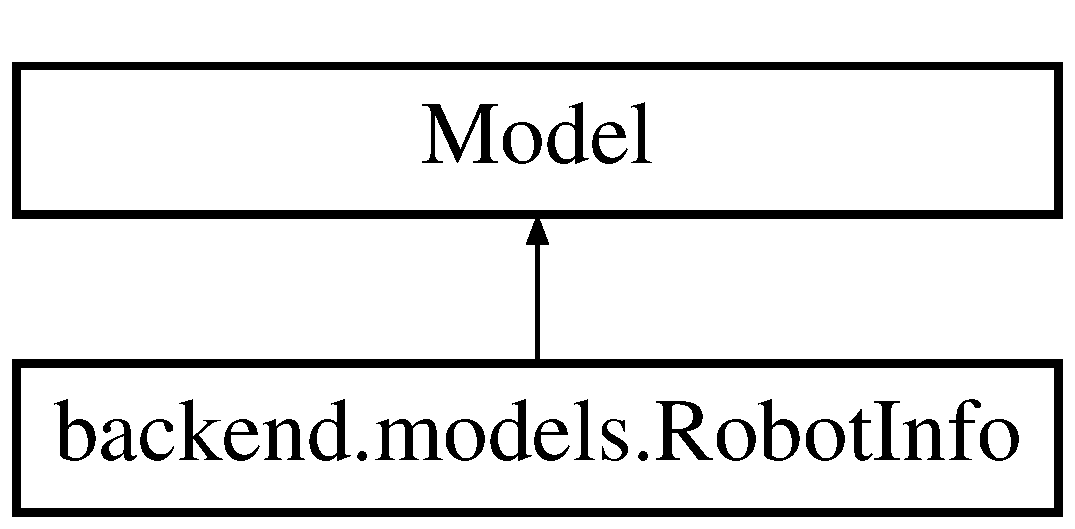
\includegraphics[height=2.000000cm]{classbackend_1_1models_1_1_robot_info}
\end{center}
\end{figure}
\subsection*{Static Public Attributes}
\begin{DoxyCompactItemize}
\item 
\mbox{\Hypertarget{classbackend_1_1models_1_1_robot_info_ad94ac4dccba02edbc9043cafa0e56688}\label{classbackend_1_1models_1_1_robot_info_ad94ac4dccba02edbc9043cafa0e56688}} 
{\bfseries enterprise} = models.\+Foreign\+Key(\textquotesingle{}\hyperlink{classbackend_1_1models_1_1_admin}{Admin}\textquotesingle{}, on\+\_\+delete=models.\+C\+A\+S\+C\+A\+DE)
\item 
\mbox{\Hypertarget{classbackend_1_1models_1_1_robot_info_a215162cb88ee5c0b6239568b019da392}\label{classbackend_1_1models_1_1_robot_info_a215162cb88ee5c0b6239568b019da392}} 
{\bfseries question} = models.\+Char\+Field(max\+\_\+length=150, default=\textquotesingle{}empty\textquotesingle{})
\item 
\mbox{\Hypertarget{classbackend_1_1models_1_1_robot_info_a3ade5f91fe1db2885f17d459104e8d44}\label{classbackend_1_1models_1_1_robot_info_a3ade5f91fe1db2885f17d459104e8d44}} 
{\bfseries answer} = models.\+Char\+Field(max\+\_\+length=500, default=\textquotesingle{}empty\textquotesingle{})
\item 
\mbox{\Hypertarget{classbackend_1_1models_1_1_robot_info_aaed612185a4a357b374f3da4f2bb5a52}\label{classbackend_1_1models_1_1_robot_info_aaed612185a4a357b374f3da4f2bb5a52}} 
{\bfseries keyword} = models.\+Char\+Field(max\+\_\+length=100, default=\textquotesingle{}empty\textquotesingle{}, blank=True)
\item 
\mbox{\Hypertarget{classbackend_1_1models_1_1_robot_info_a4ad76dafa749231ae4f858cf243af26b}\label{classbackend_1_1models_1_1_robot_info_a4ad76dafa749231ae4f858cf243af26b}} 
{\bfseries weight} = models.\+Integer\+Field(default=1)
\end{DoxyCompactItemize}


The documentation for this class was generated from the following file\+:\begin{DoxyCompactItemize}
\item 
models.\+py\end{DoxyCompactItemize}

\hypertarget{classbackend_1_1serializers_1_1_robot_info_serializer}{}\section{backend.\+serializers.\+Robot\+Info\+Serializer Class Reference}
\label{classbackend_1_1serializers_1_1_robot_info_serializer}\index{backend.\+serializers.\+Robot\+Info\+Serializer@{backend.\+serializers.\+Robot\+Info\+Serializer}}
Inheritance diagram for backend.\+serializers.\+Robot\+Info\+Serializer\+:\begin{figure}[H]
\begin{center}
\leavevmode
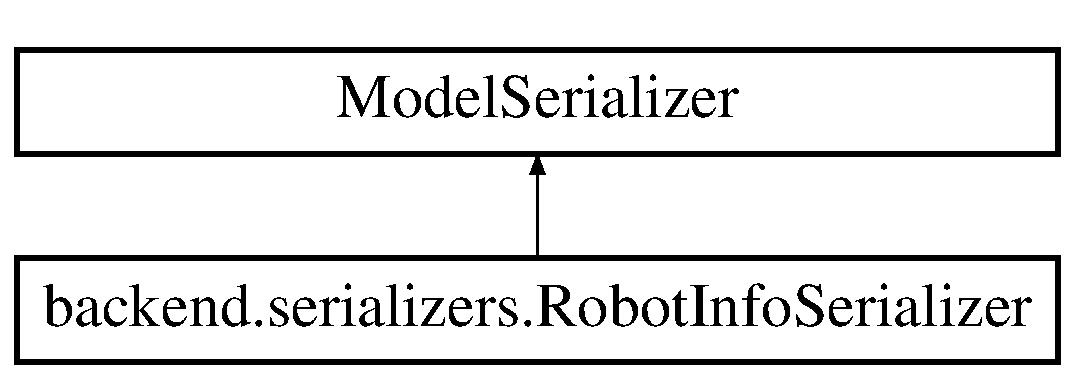
\includegraphics[height=2.000000cm]{classbackend_1_1serializers_1_1_robot_info_serializer}
\end{center}
\end{figure}
\subsection*{Classes}
\begin{DoxyCompactItemize}
\item 
class \hyperlink{classbackend_1_1serializers_1_1_robot_info_serializer_1_1_meta}{Meta}
\end{DoxyCompactItemize}


The documentation for this class was generated from the following file\+:\begin{DoxyCompactItemize}
\item 
serializers.\+py\end{DoxyCompactItemize}

\hypertarget{classbackend_1_1models_1_1_serial_number}{}\section{backend.\+models.\+Serial\+Number Class Reference}
\label{classbackend_1_1models_1_1_serial_number}\index{backend.\+models.\+Serial\+Number@{backend.\+models.\+Serial\+Number}}
Inheritance diagram for backend.\+models.\+Serial\+Number\+:\begin{figure}[H]
\begin{center}
\leavevmode
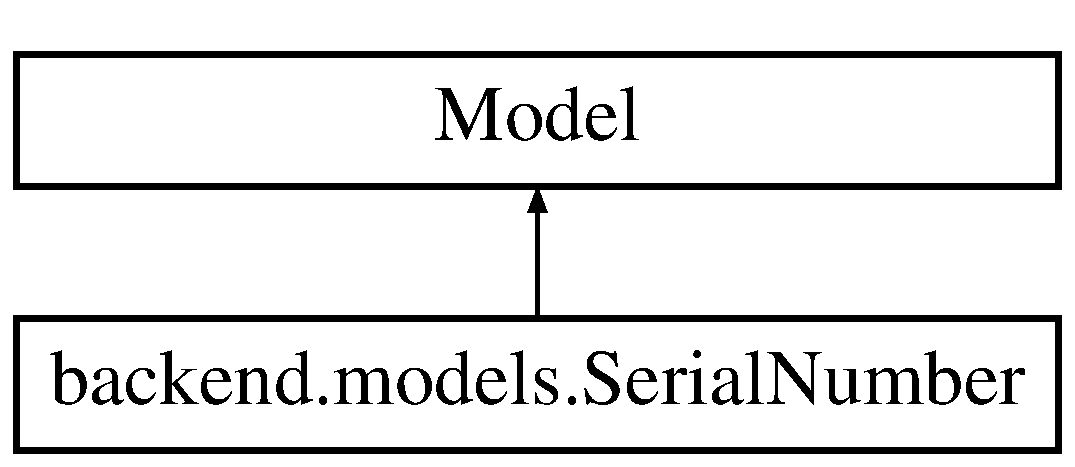
\includegraphics[height=2.000000cm]{classbackend_1_1models_1_1_serial_number}
\end{center}
\end{figure}
\subsection*{Static Public Attributes}
\begin{DoxyCompactItemize}
\item 
\mbox{\Hypertarget{classbackend_1_1models_1_1_serial_number_a1340ce7cac3c62e98d1e5dd0678fbd64}\label{classbackend_1_1models_1_1_serial_number_a1340ce7cac3c62e98d1e5dd0678fbd64}} 
{\bfseries serials} = models.\+Char\+Field(max\+\_\+length=50, default=\textquotesingle{}empty\textquotesingle{}, unique=True)
\item 
\mbox{\Hypertarget{classbackend_1_1models_1_1_serial_number_a681639e029fcd8bfd11ffd78137d5eb1}\label{classbackend_1_1models_1_1_serial_number_a681639e029fcd8bfd11ffd78137d5eb1}} 
{\bfseries is\+\_\+used} = models.\+Boolean\+Field(default=None)
\end{DoxyCompactItemize}


The documentation for this class was generated from the following file\+:\begin{DoxyCompactItemize}
\item 
models.\+py\end{DoxyCompactItemize}

\hypertarget{classbackend_1_1serializers_1_1_serial_number_serializer}{}\section{backend.\+serializers.\+Serial\+Number\+Serializer Class Reference}
\label{classbackend_1_1serializers_1_1_serial_number_serializer}\index{backend.\+serializers.\+Serial\+Number\+Serializer@{backend.\+serializers.\+Serial\+Number\+Serializer}}
Inheritance diagram for backend.\+serializers.\+Serial\+Number\+Serializer\+:\begin{figure}[H]
\begin{center}
\leavevmode
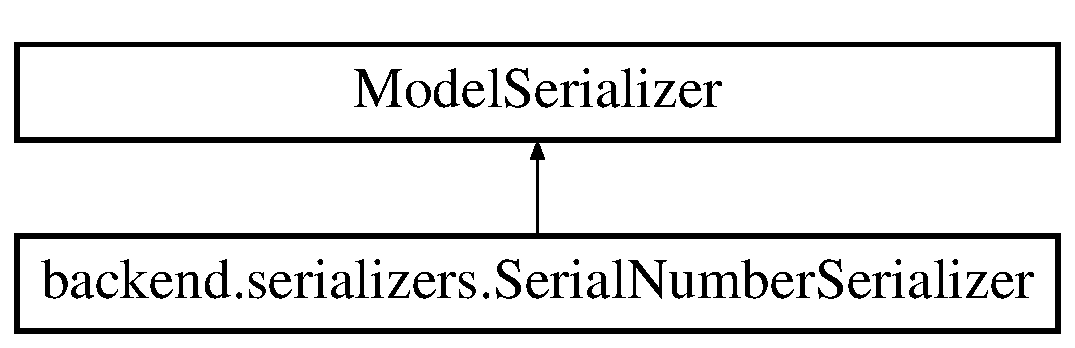
\includegraphics[height=2.000000cm]{classbackend_1_1serializers_1_1_serial_number_serializer}
\end{center}
\end{figure}
\subsection*{Classes}
\begin{DoxyCompactItemize}
\item 
class \hyperlink{classbackend_1_1serializers_1_1_serial_number_serializer_1_1_meta}{Meta}
\end{DoxyCompactItemize}


The documentation for this class was generated from the following file\+:\begin{DoxyCompactItemize}
\item 
serializers.\+py\end{DoxyCompactItemize}

\hypertarget{classbackend_1_1models_1_1_small_image_log}{}\section{backend.\+models.\+Small\+Image\+Log Class Reference}
\label{classbackend_1_1models_1_1_small_image_log}\index{backend.\+models.\+Small\+Image\+Log@{backend.\+models.\+Small\+Image\+Log}}
Inheritance diagram for backend.\+models.\+Small\+Image\+Log\+:\begin{figure}[H]
\begin{center}
\leavevmode
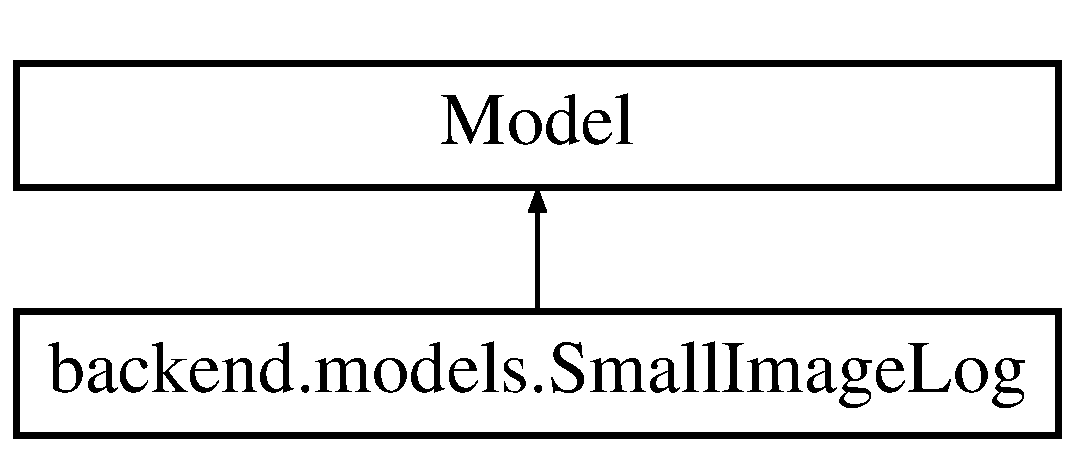
\includegraphics[height=2.000000cm]{classbackend_1_1models_1_1_small_image_log}
\end{center}
\end{figure}
\subsection*{Static Public Attributes}
\begin{DoxyCompactItemize}
\item 
\mbox{\Hypertarget{classbackend_1_1models_1_1_small_image_log_a2cac482f913dec988f5614fcaf8cff29}\label{classbackend_1_1models_1_1_small_image_log_a2cac482f913dec988f5614fcaf8cff29}} 
{\bfseries client\+\_\+id} = models.\+Char\+Field(max\+\_\+length=100, default=\textquotesingle{}empty\textquotesingle{})
\item 
\mbox{\Hypertarget{classbackend_1_1models_1_1_small_image_log_a4ee0d9d7b602c9a4fbc809c515f71e54}\label{classbackend_1_1models_1_1_small_image_log_a4ee0d9d7b602c9a4fbc809c515f71e54}} 
{\bfseries service\+\_\+id} = models.\+Foreign\+Key(\textquotesingle{}\hyperlink{classbackend_1_1models_1_1_customer_service}{Customer\+Service}\textquotesingle{}, on\+\_\+delete=models.\+C\+A\+S\+C\+A\+DE)
\item 
\mbox{\Hypertarget{classbackend_1_1models_1_1_small_image_log_a68fa2e6c5d170c774c85b8f183eff977}\label{classbackend_1_1models_1_1_small_image_log_a68fa2e6c5d170c774c85b8f183eff977}} 
{\bfseries image} = models.\+Image\+Field(upload\+\_\+to=\hyperlink{classbackend_1_1models__helper__functions_1_1_path_and_rename}{Path\+And\+Rename}(\textquotesingle{}user\+\_\+image/Small/\{\}\textquotesingle{}.format(time.\+strftime(\char`\"{}\%Y/\%m/\%d\char`\"{}))))
\item 
\mbox{\Hypertarget{classbackend_1_1models_1_1_small_image_log_a5fbf065613b02341e408275708b3af8d}\label{classbackend_1_1models_1_1_small_image_log_a5fbf065613b02341e408275708b3af8d}} 
{\bfseries extention} = models.\+Char\+Field(max\+\_\+length=10, default=\textquotesingle{}empty\textquotesingle{})
\item 
\mbox{\Hypertarget{classbackend_1_1models_1_1_small_image_log_a377bbf97d5fc4e4797487c02a6e3906c}\label{classbackend_1_1models_1_1_small_image_log_a377bbf97d5fc4e4797487c02a6e3906c}} 
{\bfseries is\+\_\+client} = models.\+Boolean\+Field(default=None)
\item 
\mbox{\Hypertarget{classbackend_1_1models_1_1_small_image_log_a6e6e006fa871d0ae6716b24d60c54a42}\label{classbackend_1_1models_1_1_small_image_log_a6e6e006fa871d0ae6716b24d60c54a42}} 
{\bfseries time} = models.\+Date\+Time\+Field(auto\+\_\+now\+\_\+add=True)
\item 
\mbox{\Hypertarget{classbackend_1_1models_1_1_small_image_log_a2459433e63e3526c8cfeac1a9160a87b}\label{classbackend_1_1models_1_1_small_image_log_a2459433e63e3526c8cfeac1a9160a87b}} 
{\bfseries label} = models.\+Char\+Field(max\+\_\+length=100, default=\textquotesingle{}empty\textquotesingle{})
\end{DoxyCompactItemize}


The documentation for this class was generated from the following file\+:\begin{DoxyCompactItemize}
\item 
models.\+py\end{DoxyCompactItemize}

\hypertarget{classbackend_1_1serializers_1_1_small_image_log_serializer}{}\section{backend.\+serializers.\+Small\+Image\+Log\+Serializer Class Reference}
\label{classbackend_1_1serializers_1_1_small_image_log_serializer}\index{backend.\+serializers.\+Small\+Image\+Log\+Serializer@{backend.\+serializers.\+Small\+Image\+Log\+Serializer}}
Inheritance diagram for backend.\+serializers.\+Small\+Image\+Log\+Serializer\+:\begin{figure}[H]
\begin{center}
\leavevmode
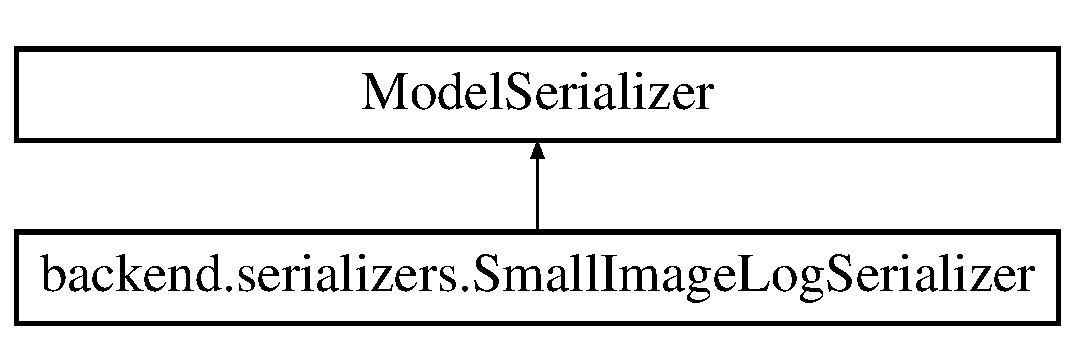
\includegraphics[height=2.000000cm]{classbackend_1_1serializers_1_1_small_image_log_serializer}
\end{center}
\end{figure}
\subsection*{Classes}
\begin{DoxyCompactItemize}
\item 
class \hyperlink{classbackend_1_1serializers_1_1_small_image_log_serializer_1_1_meta}{Meta}
\end{DoxyCompactItemize}
\subsection*{Static Public Attributes}
\begin{DoxyCompactItemize}
\item 
\mbox{\Hypertarget{classbackend_1_1serializers_1_1_small_image_log_serializer_af3bdc119361024f5f88487445ea21ad2}\label{classbackend_1_1serializers_1_1_small_image_log_serializer_af3bdc119361024f5f88487445ea21ad2}} 
{\bfseries image} = Base64\+Image\+Field()
\end{DoxyCompactItemize}


The documentation for this class was generated from the following file\+:\begin{DoxyCompactItemize}
\item 
serializers.\+py\end{DoxyCompactItemize}

%--- End generated contents ---

% Index
\backmatter
\newpage
\phantomsection
\clearemptydoublepage
\addcontentsline{toc}{chapter}{Index}
\printindex

\end{document}
